%Auteur : Nicolas Englebert
\documentclass[british,french,11pt, a4paper, openany]{book}

% Règles de bonne pratiques :
% https://fr.wikibooks.org/wiki/LaTeX/Gestion_des_gros_documents

%%%%%%%%%%%%%%%%%
%%% Packages %%%
%%%%%%%%%%%%%%%%

%%% Compatibilité %%%
\begingroup\expandafter\expandafter\expandafter\endgroup
\expandafter\ifx\csname IncludeInRelease\endcsname\relax
\usepackage{fixltx2e}
\fi 					% Si version LaTeX < 2015, inclut un fix.

%%% Général %%%
\usepackage[utf8]{inputenc}
\usepackage{babel}
\usepackage{lmodern}
\usepackage[T1]{fontenc}
\addto\extrasfrench{\sisetup{locale = FR,detect-all}} % Switch siunitx en fonction de la langue babel :)
\addto\extrasbritish{\sisetup{locale = UK,detect-all}}
\usepackage{courier}
\usepackage{graphicx}
%\usepackage{cancel}

%%% Tableau %%%
%\usepackage{tabularx} %Permet d'auto dimensionner les tableaux



%%% Bibliographie %%%
%\usepackage[style=alphabetic,backend=biber]{biblatex}
\usepackage[autostyle]{csquotes}
%\DeclareNameAlias{sortname}{last-first}
%\DeclareFieldFormat{url}{\space\url{#1}}
%\DeclareNameAlias{labelname}{last-first}
%\addbibresource{sample.bib}


%%% Graphiques %%%
%\usepackage{tikz}
%\usepackage{pgfplots}
%\usepackage{circuitikz}

%%% Mise en page %%%
\usepackage{mathtools}
\usepackage{amssymb}
\usepackage{bbm}
\usepackage{amsthm}
%\usepackage[tt]{titlepic}% Centre le titre
%\usepackage{fancyhdr}   % Permet de modifier l'entête & footer
\usepackage{caption}     % Permet d'ajouter des légendes en images sans les mettre en float + dans la marge + ref vers le haut de l'envirronement
\usepackage{wrapfig}
\usepackage{fullpage}
%\usepackage{multicol}   % pour les liste sur plusieurs colonnes
%\usepackage{subfigure}  % alligne deux images cote a cote
\usepackage{float}      %permet de mettre du texte entre les figures grace a [H]. Génial! 
\usepackage{eso-pic}    % Fond d'écran page de garde
\usepackage{adjustbox}  % Empêche les box de sortir de la page


%%% Math %%%
%\usepackage{delarray} % Belles matrices
\usepackage{siunitx}


%%% Codes %%%
%\usepackage{listings}
%\usepackage[final]{pdfpages} %% Inclusion fichier pdf

%% Reference
\usepackage{hyperref}
%\renewcommand*{\figureautorefname}{fig.}
%\def\appendixautorefname{annexe}
%\def\tableautorefname{tab.}
%\renewcommand*{\chapterautorefname}{ch.}
%\newcommand{\subfigureautorefname}{\figureautorefname}



%%%%%%%%%%%%%%%%%
%%% Commandes %%%
%%%%%%%%%%%%%%%%%

%%% Physique %%%
\newcommand{\cst}{\text{cst}}
\newcommand{\D}{\partial}
\newcommand{\E}{\vec E}
\newcommand{\B}{\vec B}
\newcommand{\F}{\vec F}
\newcommand{\modu}[1]{|$#1$|}

%%% Math %%%
\newcommand{\oiint}{\int\!\!\!\!\!\!\! \:\!\subset\!\!\supset\!\!\!\!\!\!\!\int}
\newcommand{\rot}{\operatorname{\vec{rot}}}
\newcommand{\divv}{\operatorname{div}}
\newcommand{\phas}[1]{\underline{#1}}
\newcommand{\RE}{\text{Re}}
\newcommand{\ft}{\overset{\mathcal{F}}{\longleftrightarrow}}
\newcommand{\lt}{\overset{\mathcal{L}}{\longleftrightarrow}}
\newcommand{\DS}{\displaystyle}
\newcommand{\Tr}{\operatorname{Tr}}



%% Box
\shorthandon{:}
\newcommand{\theor}[1]{\adjustbox{minipage=\linewidth-2\fboxsep-2\fboxrule,fbox}{\textsc{\iflanguage{british}{Theorem}{Théorème}: }#1}}
\newcommand{\defi}[1]{\adjustbox{minipage=\linewidth-2\fboxsep-2\fboxrule,fbox}{\textsc{\iflanguage{british}{Definition}{Définition}: }#1}}
\newcommand{\lemme}[1]{\adjustbox{minipage=\linewidth-2\fboxsep-2\fboxrule,fbox}{\textsc{\iflanguage{british}{Lemma}{Lemme}: }#1}}
\newcommand{\prop}[1]{\adjustbox{minipage=\linewidth-2\fboxsep-2\fboxrule,fbox}{\textsc{\iflanguage{british}{Property}{Propriété}}\\ #1}}
\newcommand{\proposition}[1]{\adjustbox{minipage=\linewidth-2\fboxsep-2\fboxrule,fbox}{\textsc{Proposition}\\#1}}
\newcommand{\cadre}[1]{\adjustbox{minipage=\linewidth-2\fboxsep-2\fboxrule,fbox}{#1}}
\newcommand{\retenir}[1]{\adjustbox{minipage=\linewidth-2\fboxsep-2\fboxrule,fbox}{\textbf{\textit{\textsc{\iflanguage{british}{To remember}{À retenir}}: }}#1}}

\newcommand{\corollaire}[1]{\bigbreak\begin{tabular}{||c}
	\begin{minipage}{\textwidth}
		\textsc{\iflanguage{british}{Corollary}{Corollaire}: } \textit{#1}
	\end{minipage}
	\end{tabular}}
\newcommand{\exemple}[1]{\bigbreak\begin{tabular}{|c}
	\begin{minipage}{\textwidth}
		\textsc{\iflanguage{british}{Example}{Exemple}: } #1
	\end{minipage}%
	\end{tabular}}%
\shorthandoff{:}
    

%\pagestyle{headings} % Titre du ch et numéro page dans l'entete
%\renewcommand{\proofname}{Démonstration}
%\addto\captionsfrench{\def\tablename{Tableau}}


%%% Background %%%
\newcommand\BackgroundPic{%
	\put(0,0){%
		\parbox[b][\paperheight]{\paperwidth}{%
			\vfill
			\centering
			\includegraphics[width=\paperwidth,height=\paperheight,%
			keepaspectratio]{../../Builder/ulb.jpg}%
			\vfill
}}}

%%% Annexes Cedu %%%
%\usepackage{calrsfs}
%\DeclareMathAlphabet{\pazocal}{OMS}{zplm}{m}{n}
\usepackage{fourier-orns}

\setlength{\parindent}{0pt} 

%%% Attributs %%%
\newcommand*{\NomduCours}[2]{\def\cours{#1}\def\memo{#2}}
\newcommand*{\annee}[2]{\def\adebut{#1}\def\afin{#2}}

\newcounter{auteurcnt}
\newcommand\addauteur[2]{%
	\stepcounter{auteurcnt}%
	\csdef{auteur\theauteurcnt}{\mbox{#1~\textsc{#2}}}}
\newcommand\getauteur[1]{%
	\csuse{auteur#1}}

\newcounter{illustrateurcnt}
\newcommand\addillustrateur[2]{%
	\stepcounter{illustrateurcnt}%
	\csdef{illustrateur\theillustrateurcnt}{\mbox{#1~\textsc{#2}}}}
\newcommand\getillustrateur[1]{%
	\csuse{illustrateur#1}}

\newcounter{rappeltheocnt}
\newcommand\addrappeltheo[2]{%
	\stepcounter{rappeltheocnt}%
	\csdef{rappeltheo\therappeltheocnt}{\mbox{#1~\textsc{#2}}}}
\newcommand\getrappeltheo[1]{%
	\csuse{rappeltheo#1}}

\newcounter{professeurcnt}
\newcommand\addprofesseur[2]{%
	\stepcounter{professeurcnt}%
	\csdef{professeur\theprofesseurcnt}{\mbox{#1~\textsc{#2}}}}
\newcommand\getprofesseur[1]{%
	\csuse{professeur#1}}

\newcounter{iter}
%\usepackage{ulem}
%Typique Phys
\usepackage{../../Builder/preambule}
\usepackage{cancel,physics}
% Attributs
\NomduCours{Mécanique quantique II}{PHYS-H401}
\addauteur{Nicolas}{Englebert}
\addprofesseur{Nicolas}{Cerf}
\annee{2016}{2017}


% Document
\begin{document}
\def\equationautorefname~#1\null{%
	(#1)\null
}
%%%%%%%%%%%%%%%%%
% Préliminaires %
%%%%%%%%%%%%%%%%%
\frontmatter
\input{../../Builder/titlepage/titlepage.tex}
\ \\[2cm]
{\Huge \bfseries Appel à contribution}\\[5mm]
\subsection*{Synthèse Open Source}
\begin{wrapfigure}[5]{l}{4.5cm}
	\includegraphics[scale=0.5]{../../Builder/git.png}
\end{wrapfigure}
Ce document est grandement inspiré de l’excellent cours donné 
par \ifnum\theprofesseurcnt=1 \getprofesseur{1} \else\whileboolexpr
{ test {\ifnumcomp{\value{iter}}{<}{\theprofesseurcnt-2}} }%
{\stepcounter{iter}\getprofesseur{\theiter}, }%
\stepcounter{iter}\getprofesseur{\theiter} et \stepcounter{iter}\getprofesseur{\theiter} \fi%
 à l’EPB (École Polytechnique de Bruxelles), faculté de l’ULB (Université 
Libre de Bruxelles). Il est écrit par les auteurs susnommés avec l’aide de tous les autres étudiants 
et votre aide est la bienvenue ! En effet, il y a toujours moyen de l’améliorer surtout que si le 
cours change, la synthèse doit être changée en conséquence. On peut retrouver le code source à l’adresse 
suivante
\begin{center}
	\url{https://github.com/nenglebert/Syntheses}
\end{center}\bigskip
Pour contribuer à cette synthèse, il vous suffira de créer un compte sur \textit{Github.com}. De
légères modifications (petites coquilles, orthographe, ...) peuvent directement être faites sur le
site ! Vous avez vu une petite faute ? Si oui, la corriger de cette façon ne prendra que quelques 
secondes, une bonne raison de le faire ! \bigskip

Pour de plus longues modifications, il est intéressant de disposer des fichiers : il vous 
faudra pour cela installer \LaTeX, mais aussi \textit{git}. Si cela pose problème, nous sommes 
évidemment ouverts à des contributeurs envoyant leur changement par mail ou n’importe quel autre 
moyen.\bigskip

Le lien donné ci-dessus contient aussi un \texttt{README} contenant de plus amples informations, 
vous êtes invités à le lire si vous voulez faire avancer ce projet ! 

\subsection*{Licence Creative Commons}
\begin{wrapfigure}[3]{r}{2.8cm}
	\vspace{-5mm}
	\includegraphics[scale=0.17]{../../Builder/CC}
\end{wrapfigure}
Le contenu de ce document est sous la licence Creative Commons : \textit{Attribution-NonCommercial-ShareAlike 
4.0 International (CC BY-NC-SA 4.0)}. Celle-ci vous autorise à l'exploiter pleinement, compte-
tenu de trois choses :
\begin{enumerate}
	\item \textit{Attribution} ; si vous utilisez/modifiez ce document vous devez signaler le(s) nom(s)
	      de(s) auteur(s).
	\item \textit{Non Commercial} ; interdiction de tirer un profit commercial de l’œuvre sans 
	      autorisation de l'auteur 
	\item \textit{Share alike} ;  partage de l’œuvre, avec obligation de rediffuser selon la même 
	      licence ou une licence similaire
\end{enumerate}
Si vous voulez en savoir plus sur cette licence :
\begin{center}
	\url{http://creativecommons.org/licenses/by-nc-sa/4.0/}
\end{center}

\begin{flushright}
	\textbf{Merci ! }
\end{flushright}
\tableofcontents
%Si abstract, \input ici

%%%%%%%%%%%%%%%%%%%%%
% Contenu principal %
%%%%%%%%%%%%%%%%%%%%%
\mainmatter
\chapter{Systèmes hydrogénoïdes: structures fines et hyperfines}
\section{Équation de Schrödinger (rappel)}
	\begin{wrapfigure}[9]{r}{4cm}
	\vspace{-18mm}
	\includegraphics[scale=0.4]{ch1/image1}
	\captionof{figure}{ }
	\end{wrapfigure}
Avant toute chose, signalons que ce chapitre (ainsi que le suivant) est grandement inspiré
de \textit{Physics of Atomes and Molecules} de \textsc{B.H. Bransden} et \textsc{C.J.
Joachain}. Commençons par rappeler le système de coordonnées sphérique
\begin{equation}
\left\{\begin{array}{ll}
x &= r\sin\theta\cos\phi\\
y &= r\sin\theta\sin\phi\\
z &= r\cos\theta
\end{array}\right.
\end{equation}
Il convient de ne pas oublier le jacobien lors du changement de variable
\begin{equation}
d\vec{r} = dxdydz : (r\sin\theta d\phi)(rd\theta)dr = r^2\sin\theta drd\theta d\phi
\end{equation}

\subsection{Les harmoniques sphériques}
Le moment cinétique orbital $\vec{L}$ au carré s'écrit
\begin{equation}
\vec{L}^2 = \vec{L}.\vec L = L^2_x+L^2_y+L^2_z
\end{equation}
En coordonnée sphériques
\begin{equation}
\vec L^2 = -\hbar^2\left[\frac{1}{\sin\theta}\frac{\partial}{\partial \theta}\left(\sin\theta\frac{\partial}{
\partial \theta}\right)+\frac{1}{\sin^2\theta}\frac{\partial^2}{\partial\phi^2}\right]
\end{equation}
Les \textbf{harmoniques sphériques} sont par définition fonction propres de $\vec{L}^2$, mais aussi $L_z$\\

\cadre{\begin{equation}
\begin{array}{ll}
\vec{L}^2Y_{lm}(\theta,\phi) &= \hbar^2l(l+1)Y_{lm}(\theta,\phi)\\
L_z Y_{lm}(\theta,\phi) &= \hbar mY_{lm}(\theta,\phi)
\end{array}
\end{equation}
où $l=0,1,2,3,\dots$ et $m= l,l-1,l-2,\dots, -l$.}\ \\

Le choix de $m$ (pour \textit{magnétique}) prendra tout son sens lorsque l'on plongera le système dans un 
champ magnétique et que l'on perdra la symétrie sphérique par le fait qu'il existe une direction privilégiée. 
Comme ces deux observables ont des fonctions propres communes, elles doivent forcément commuter
\begin{equation}
[\vec{L}^2, L_z] = 0
\end{equation}
Pour nommer les orbitales, on donne un doux nom à chaque valeur de $l$\\

\cadre{$$l=0,1,2,3,4,5,6,7,\dots$$ $$s,p,d,f,h,i,k,\dots$$
où la lettre $j$ a volontairement été laissée sur le côté pour ne pas la confondre avec de $i$, ce qui 
pouvait facilement être le cas en utilisant des machines à écrire !}\ \\

Pour les retenir, un petit moyen mnémotechnique : \textit{"\textbf{S}olar \textbf{P}hysicists \textbf{D}on't
\textbf{F}ind \textbf{G}iraffes \textbf{H}idding \textbf{I}n \textbf{K}itchens}.\\

Les harmoniques sphériques sont définies pour $m \geq 0$ par 
\begin{equation}
Y_{lm} (\theta, \phi) = (-1)^m
\left[ \frac{(2l+1)}{4 \pi} \frac{(l-m)!}{(l+m)!}
\right] ^{\frac{1}{2}}  P^{m}_l (\cos \theta) e^{i m \phi}
\end{equation}
Dans le cas où $m$ est négatif, on trouve l'harmonique sphérique associée via : 
\begin{equation}
Y_{l,-m} (\theta, \phi) = (-1)^m Y^\ast_{lm} (\theta, \phi)
\end{equation}
Les harmoniques sphériques répondent aux relations d'orthonormalité, où il convient de ne pas oublier le 
facteur en $\theta$. Le prix à payer est bien évidemment celui de la normalisation :
\begin{equation}
\int_0^\pi d \theta \sin \theta 
\int_0^{2 \pi} d\phi \; Y_{lm}^\ast (\theta,\phi) \; 
Y_{l'm'} (\theta,\phi) = \delta_{ll'} \delta_{mm'}
\end{equation}

On peut définir des opérateurs de montée et de descente
\begin{equation}
L_+ \equiv L_x+iL_y,\qquad\qquad\qquad\qquad L_- \equiv L_x-iL_y
\end{equation}
Avec ceux-ci, il est possible de modifier la valeur de la projection du nombre quantique $l$, c'est-à-dire
$m_l$ (ou encore, $m$)
\begin{equation}
L_\pm Y_{lm}(\theta,\phi) = \hbar\sqrt{l(l+1)-m(m\pm 1)}Y_{lm\pm1}(\theta,\phi)
\end{equation}
\newpage
Suivant cette définition, voici quelques harmoniques sphériques 
\begin{equation}
\begin{array}{l}
 Y_{0,0} = \frac{1}{(4 \pi)^{1/2}}  \\
\ \\
 Y_{1,0} = \left( \frac{3}{4 \pi} \right)^{1/2} \cos \theta \\
 Y_{1,\pm 1}  = \mp \left( \frac{3}{8 \pi} \right)^{1/2} \sin \theta \; e^{\pm i \phi} \\
\ \\
 Y_{2,0} = \left( \frac{5}{16 \pi} \right)^{1/2} (3 \cos^2 \theta - 1)   \\
 Y_{2,\pm 1} = \mp \left( \frac{15}{8 \pi} \right)^{1/2} \sin \theta \cos \theta \; e^{\pm i \phi} \\
 Y_{2,\pm 2} = \left( \frac{15}{32 \pi} \right)^{1/2} \sin^2 \theta \; e^{\pm 2i \phi} \\
\ \\
 Y_{3,0} = \left( \frac{7}{16 \pi} \right)^{1/2}   (5 \cos^3 \theta - 3 \cos \theta)  \\
 Y_{3,\pm 1} = \mp \left( \frac{21}{64 \pi} \right)^{1/2}    \sin \theta (5 \cos^2 \theta - 1)  \; e^{\pm i \phi} \\
 Y_{3,\pm 2} =  \left( \frac{105}{32\pi} \right)^{1/2}    \sin^2 \theta \cos \theta \; e^{\pm 2 i \phi} \\
 Y_{3,\pm 3} = \mp \left( \frac{35}{64 \pi} \right)^{1/2}    \sin^3 \theta  \; e^{\pm 3 i \phi}
\end{array}
\end{equation}



\subsection{Les forces centrales}
Un potentiel central est un potentiel présentant une symétrie sphérique
\begin{equation}
V(\vec{r}) = V(r)
\end{equation}
où $r = |\vec r|$. Pour traiter ce potentiel de façon efficace, il convient d'écrire l'Hamiltonien 
\begin{equation}
H = -\frac{\hbar^2}{2m}\nabla^2+V(r)
\end{equation}
en coordonnées sphériques
\begin{equation}
H = -\frac{\hbar^2}{2m}\left[\frac{1}{r^2}\frac{\partial}{\partial r}\left(r^2\frac{\partial}{\partial r}\right)
+\frac{1}{r^2\sin\theta}\frac{\partial}{\partial \theta}\left(\sin\theta\frac{\partial}{\partial \theta}\right)
+ \frac{1}{r^2\sin^2\theta}\frac{\partial^2}{\partial \phi^2}\right] + V(r)
\end{equation}
En utilisant l'écriture sphérique de $\vec{L}^2$
\begin{equation}
\vec L^2 = -\hbar^2\left[\frac{1}{\sin\theta}\frac{\partial}{\partial \theta}\left(\sin\theta\frac{\partial}{
\partial \theta}\right)+\frac{1}{\sin^2\theta}\frac{\partial^2}{\partial\phi^2}\right]
\end{equation}
On peut écrire l'Hamiltonien sous une forme sphérique
\begin{equation}
H=-\frac{\hbar^2}{2m}\left[\frac{1}{r^2}\frac{\partial}{\partial r}\left(r^2\frac{\partial}{\partial r}\right)
-\frac{\vec L^2}{\hbar^2 r^2}\right] + V(r)
\end{equation}
Cet Hamiltonien vérifie les relations de commutation suivante
\begin{equation}
[H,\vec{L}^2] = [H,L_z] = [\vec{L}^2,L_z] = 0
\end{equation}
Il est possible de résoudre l'équation de Schrödinger par la méthode de séparation des variables, à l'aide
de nos harmoniques sphériques
\begin{equation}
\psi_{E,l,m}(r,\theta,\phi) = R_{E,l}(r)Y_{lm}(\theta,\phi)
\end{equation}
On peut alors obtenir l'équation radiale
\begin{equation}
\left\{-\frac{\hbar^2}{2m}\left[\frac{1}{r^2}\frac{d}{dr}\left(r^2\frac{d}{dr}\right) - \frac{l(l+1)}{r^2}\right]+
V(r)\right\}R_{E,l}(r) = ER_{E,l}(r)
\end{equation}
En effectuant le changement de variable $P_{E,l}(r) \equiv rR_{E,l}(r)$, on retrouve une équation de 
Schrödinger sous un format "classique"
\begin{equation}
\left[-\frac{\hbar^2}{2m}\frac{d^2}{dr^2}+\frac{\hbar^2l(l+1)}{2mr^2}+V(r)\right]P_{E,l}(r) = EP_{E,l}(r)
\end{equation}
On retiendra le comportement asymptotique suivant, pour $r\to0$ : $P_{E,l}(r) \sim r^{l+1}$.\\


La fonction factorisée $\psi_{E,l,m}(r,\theta,\phi) = R_{E,l}(r)Y_{lm}(\theta,\phi)$ respecte les règles 
d'inversion et de parité. On défini l'opération d'inversion (ou parité)
\begin{equation}
I\psi_{E,l,m}(\vec{r}) = I\psi_{E,l,m}(-\vec{r})
\end{equation}
Comme $I = I^\dagger$, ses valeurs propres sont réelles. Grâce à sa commutation avec l'Hamiltonien, on peut
écrire
\begin{equation}
[H,I]=0\Rightarrow I\psi_{E,l,m}(r)=\alpha\psi_{E,l,m}(r)
\end{equation}
Comme $I^2=E$, il en vient que $\alpha^2$ est forcément l'unité. Dès lors, $\alpha = \pm1$. Ceci revient à 
effectuer le changement de variable suivant (en cartésien et sphérique)
\begin{equation}
\left\{\begin{array}{ll}
x &\to -x\\
y &\to -y\\
z &\to -z
\end{array}\right. \qquad\qquad\qquad\left\{\begin{array}{ll}
r &\to -r\\
\theta &\to (\pi-\theta)\\
\phi &\to (\phi+\pi)
\end{array}\right. 
\end{equation}
Appliquons cet opérateur sur notre fonction factorisée :$I\psi_{E,l,m}(r,\theta,\phi) = I[R_{E,l}(r)Y_{lm}(\theta,
\phi)]$. Ceci donne
\begin{equation}
I\psi_{E,l,m}(r,\theta,\phi) = R_{E,l}(r)[IY_{lm}(\theta,\phi)] = (-1)^lR_{E,l}(r)Y_{lm}(\theta,\phi)
\end{equation}
où l'on voit apparaître la fonction factorisée. Nous avons ainsi défini l'effet de l'application de l'opérateur
parité sur la fonction d'onde \\

\cadre{
\begin{equation}
I\psi_{E,l,m}(r,\theta,\phi) = (-1)^l\psi_{E,l,m}(r,\theta,\phi)
\end{equation}}\ \\

Ainsi, $l$ pair implique $\alpha=+1$ et l'on parlera d'états \textbf{pairs}. A l'inverse, on parlera d'états
\textbf{impairs}.




\subsection{Problème à 2 corps: effet de masse}
Considérons deux particules en interaction
\begin{equation}
H = \frac{\vec p_1^2}{2m_1}+\frac{\vec p_2^2}{2m_2}+V(\vec r_1-\vec r_2)
\end{equation}
A l'aide du principe de correspondance $p\to -i\hbar\vec\nabla$ et $\vec{L}\to \vec{L}=-i\hbar(\vec{r}\times
\vec\nabla)$, on peut retrouver l'équation de Schrödinger
\begin{equation}
i\hbar\frac{\partial}{\partial t}\Psi(\vec{r}_1,\vec{r}_2, t) = \left[-\frac{\hbar^2}{2m_1}\nabla_1^2
-\frac{\hbar^2}{2m_2}\nabla_2^2+V(\vec r_1-\vec r_2)\right]\Psi(\vec{r}_1,\vec{r}_2, t)
\end{equation}
où $V$ ne dépend que de la coordonnée relative $\vec{r} =\vec{r_1}-\vec{r_2}$. Il est également pratique 
d'exprimer la coordonnée relative du centre de masse $\vec{R} = \frac{m_1\vec r_1+m_2\vec r_2}{m_1+m_2}$.
Effectuons alors le changement de coordonnées $(\vec{r_1},\vec{r_2})\to (\vec{r},\vec{R})$. Ceci peut se 
faire en définissant la masse totale et la masse réduite
\begin{equation}
M=m_1+m_2,\qquad\qquad\qquad \mu = \frac{m_1m_2}{m_1+m_2}
\end{equation}
En définissant le moment relatif $\vec{p}=\frac{m_2\vec p_1-m_1\vec p_2}{m_1+m_2}$ et le moment total $\vec{P}
= \vec{p_1}+\vec{p_2}$, nous avons que
\begin{equation}
\frac{\vec p_1^2}{2m_1}+\frac{\vec p_2^2}{2m_2} = \frac{\vec P^2}{2M}+\frac{\vec p^2}{2\mu}
\end{equation}
L'équation de Schrödinger devient
\begin{equation}
i\hbar\frac{\partial}{\partial t}\Psi(\vec R, \vec r, t) = \left[-\frac{\hbar^2}{2M}\nabla_R^2
-\frac{\hbar^2}{2\mu}\nabla_r^2+V(\vec r)\right]\Psi(\vec R, \vec r, t)
\end{equation}
où l'on voit cette fois-ci clairement apparaître la masse réduite $\mu$. Lorsque le potentiel $V$ est 
indépendant du temps $t$, il est possible d'effectuer le découplage du centre de masse et du mouvement 
relatif
\begin{equation}
\Psi(\vec R, \vec r, t) = \Phi(\vec{R})\psi(\vec{r})e^{-i(E_{CM}+E)t/\hbar}
\end{equation}
Ce découplage implique que l'on considère une particule libre de masse $M$ pour le centre de masse
\begin{equation}
-\frac{\hbar^2}{2M}\Delta_R^2\Phi(\vec{R}) = E_{CM}\Phi(\vec{R})
\end{equation}
Nous avons également à considérer une particule de masse $\mu$, cette fois-ci dans un potentiel $V(r)$
\begin{equation}
\left[-\frac{\hbar^2}{2\mu}\nabla_r^2+V(r)\right]\psi(\vec{r}) = E\psi(\vec{r})
\end{equation}
où nous retrouvons bien la masse réduite. Dans le contexte de l'atome d'hydrogène, celle-ci sera proche de la
masse de l'électron. \\

L'énergie totale à considérée est bien donnée par
\begin{equation}
E_{tot} = E_{CM}+E
\end{equation}


\subsection{Systèmes hydrogénoïdes – Potentiel de Coulomb}
Pour un système hydrogénoïde, nous devons utiliser l'équation décrivant le mouvement relatif
\begin{equation}
\left[-\frac{\hbar^2}{2\mu}\nabla_r^2+V(r)\right]\psi(\vec{r}) = E\psi(\vec{r})
\end{equation}
En utilisant comme potentiel le potentiel de \textsc{Coulomb} (potentiel central)
\begin{equation}
V(\vec{r}) = V(r) = -\dfrac{Ze^2}{4\pi\epsilon_0r}
\end{equation}
Celui-ci est le reflet d'un potentiel liant (négatif, ceci reflétant de \textsc{Coulomb} liant deux charges
opposées).

Cherchons les solutions en coordonnées sphérique $\psi_{E,l,m}(r,\theta,\phi) = R_{E,l}(r)Y_{lm}(\theta,\phi)$. 
L'équation radiale s'écrit
\begin{equation}
\left\{-\frac{\hbar^2}{2\mu}\left[\frac{1}{r^2}\frac{d}{dr}\left(r^2\frac{d}{dr}\right) - \frac{l(l+1)}{r^2}\right]+
V(r)\right\}R_{E,l}(r) = ER_{E,l}(r)
\end{equation}
où $r$ est la coordonnées relative et où ce n'est pas la masse de l'électron $m$ qui apparaît mais la masse
réduite $\mu$. C'est l'effet de masse qui apparaît lorsque les choses sont traitées correctement. Avec le 
changement de variable $P_{E,l}(r) \equiv rE_{E,l}(r)$ et en substituant , on trouve\\

\cadre{
\begin{equation}
\left[-\frac{\hbar^2}{2\mu}\frac{d^2}{dr^2}+\frac{\hbar^2l(l+1)}{2\mu r^2}-\frac{Ze^2}{4\pi\epsilon_0r}\right]P_{E,l}(r) = EP_{E,l}(r)
\end{equation}
\danger\ C'est bien la masse réduite $\mu$ qui apparaît ici.}\ \\

Cette équation permet de décrire les systèmes hydrogénoïdes, c'est-à-dire les systèmes atomiques à un seul
électron ($Z=1 : H, Z=2 : He^+, Z=91 :\  ^{91}U^{90+}, \dots$).\\


	\begin{wrapfigure}[14]{r}{4cm}
	\vspace{-5mm}
	\includegraphics[scale=0.4]{ch1/image2}
	\captionof{figure}{ }
	\end{wrapfigure}
Pour retrouver une équation de Schrödinger "classique", on définit le \textit{potentiel effectif} $V_{eff}^{(l)}$
\begin{equation}
V_{eff}^{(l)} = -\frac{Ze^2}{4\pi\epsilon_0r}+\dfrac{l(l+1)\hbar^2}{2\mu r^2}
\end{equation}
Le second terme du membre de droite est le \textit{potentiel centrifuge} qui, contrairement au potentiel
de \textsc{Coulomb}, est antiliant (signe positif). Le potentiel effectif est déterminé par la valeur de
$l$ : une valeur nulle de $l$ donne le potentiel coulombien.\\

Cependant, dès que $l\neq 0$, une nouvelle contribution à petite distance apparaît. Elle relève l'existence d'un
potentiel centrifuge qui fait que l'on a une barrière coulombienne que l'on ne retrouve pas pour $l=0$. Ceci
explique le comportement différent pour un électron $s$ ou $p$, le potentiel étant totalement différent.


\newpage
\subsection{Solution pour les états liés}
La solution de l'équation ci-dessus pour des états liés est donnée par 
\begin{equation}
E_n = -\frac{1}{2n^2}\left(\frac{Ze^2}{4\pi\epsilon_0}\right)^2\frac{\mu}{\hbar^2}=-\frac{e^2}{(4\pi\epsilon_0)
a_0}\left(\frac{\mu}{m}\right)\frac{Z^2}{2n^2}
\end{equation}
où $a_0=\frac{(4\pi\epsilon_0)\hbar^2}{me_2}$ est le rayon de \textsc{Bohr}.\\

	\begin{wrapfigure}[23]{l}{8.5cm}
	\vspace{-5mm}
	\includegraphics[scale=0.4]{ch1/image3}
	\captionof{figure}{ }
	\end{wrapfigure}
	
	Ci-contre, la représentation de la solution pour les états liés dans le cadre de l'atome d'hydrogène
	($Z=1, \mu=m$). La première chose que l'on peut constater est la présence de transition dans quasi toutes
	les classes, tout dépend de la transition regardées. On retrouve les raies de \textsc{Lyman} (transitions
	vers $n=1$), les raies de \textsc{Balmer} (transitions vers $n=2$), les raies de \textsc{Paschen}
	(transitions vers $n=3$) mais également les raies de \textsc{Brackett} (transitions vers $n=4$).\\
	
	Pour l'état $n=2$, on retrouve les états $2s_0, 2p_{+1}$ et $2p_{-1}$ qui sont tous caractérisés par
	une énergie $E_2$ donnée par la solution ci-dessus. Le niveau fondamental (énergie de 13.6 eV) n'est 
	autre que l'état $1s$. On note souvent les énergie en $cm^{-1}$, d'où l'échelle verticale. Si on regarde
	la différence entre $n=2$ et $n=1$, elle vaut à peu près $100'000$ cm$^{-1}$. Il s'agit du \textbf{
	nombre d'onde} défini comme l'inverse de la longueur d'onde. Plusieurs écritures sont possibles
	\begin{equation}
	\frac{1}{\lambda}\equiv \bar\lambda = \sigma = \bar\nu
	\end{equation}
	La longueur d'onde est l'inverse de cette "distance" et on retrouve bien la valeur de 1216 Angström. 
	Il existe une relation donnant la fréquence en fonction de la différence de l'inverse de deux nombres 
	entiers multipliée par une certaine constante afin que ce soit correction dimensionnement
	\begin{equation}
	\nu = R_\infty\left(\frac{1}{n_1^2}-\frac{1}{n_2^2}\right)\qquad\text{où }\quad R_\infty = \frac{m}{
	4\pi\hbar^3}\left(\frac{e^2}{4\pi\epsilon_0}\right)^2
	\end{equation}
	

\subsection{Système d'unités atomiques}
Le système d'unité atomique est un système horrible ou tout vaut 1. Avant de l'énoncer, rappelons la 
définition du rayon de \textsc{Bohr}
\begin{equation}
a_0=\frac{(4\pi\epsilon_0)\hbar^2}{me_2} = 5.29\times 10^{-11}\text{ m}
\end{equation}
On dira que $a_0$ = 1 u.a. de longueur. Si on veut savoir, ce que ça vaut, il faudra faire les bonnes
substitution dans la formule de $a_0$ sachant que
$m=m_e$ = 1 u.a. de masse, $e$ = 1 u.a. de charge, $\hbar$ = 1 u.a. de moment angulaire et $4\pi\epsilon_0$ =
1 u.a.  de permittivité du vide. Ce choix d'unité est fait pour déterminer avec intelligence l'énergie. Si on 
évalue l'énergie $E_n$ ci-dessus avec ces unités, presque tout va se simplifier.\\

Sachant que une unité atomique d'énergie est donnée par $E_h = e^2/(4\pi\epsilon_0 a_0)$, il est vient que
$E_n \approx -\frac{Z^2}{2n^2}E_h$. Pour $Z=1$, on trouve $E_{n=1} \approx -1/2 E_h$. Il est possible de 
retrouver la valeur sachant que $1 E_h$ (un hartree) vaut 27.2 eV.\\

Ce système simplifie également les vitesses
\begin{equation}
v_0 = \frac{e^2}{(4\pi\epsilon_0)\hbar}\equiv \alpha c = 1 \text{ u.a. de vitesse}
\end{equation}
Comme $\alpha \approx 1/137$, on en déduit que $c\approx 137$ u.a. de vitesse.\\


\subsection{Solutions pour les états liés}
Compte tenu de ce système d'unité, on peut alors ré-écrire la solution pour les états liés d'énergie $E_n$
\begin{equation}
E_n = -\frac{e^2}{(4\pi\epsilon_0)a_\mu}\frac{Z^2}{2n^2}=-\dfrac{Z^2}{2n^2}\left(\frac{\mu}{m}\right)\text{ u.a.}
\end{equation}
La fonction radiale s'écrit alors
\begin{equation}
R_{nl}(r) = P_{nl}(r) / r=
  - \left\{ \left( \frac{2Z}{na_\mu} \right)^3
   \frac{(n-l-1)!}{2n[(n+l)!]^3} \right\}^{1/2} \;
  e^{-\rho/2} \rho^l \; L^{2l+1}_{n+l} (\rho)
\end{equation}
$\mbox{o\`u}~L^{2l+1}_{n+l}(\rho)~\mbox{est un polyn\^ome de
degr\'e}~n_r = n-l-1$. On possède donc une loi d'échelle reliant $\rho$ à $r$.
\begin{equation}
\rho 
= \frac{2Z}{na_\mu} \; r, \hspace*{2cm} 
 a_\mu = \frac{4 \pi \epsilon_0 \hbar^2}{\mu e^2}
\end{equation}
Quelques exemples, pour le plaisir des yeux
\begin{equation}
\begin{array}{l}
R_{10}(r) = 2 (Z/a_0)^{3/2} \exp (-Zr/a_0) \\
\ \\
R_{20}(r) = 2 (Z/2 a_0)^{3/2} (1-Zr/2 a_0) \exp (-Zr/2 a_0) \\
R_{21}(r) = \frac{1}{\sqrt{3}}  (Z/2 a_0)^{3/2} (Zr/a_0)
        \exp (-Zr/2 a_0) \\
\ \\
R_{30}(r) = 2 (Z/3a_0)^{3/2} (1 - 2Zr/3 a_0 + 2 Z^2r^2/27a_0^2) \\
  \hspace*{4cm}  \exp(-Zr/3a_0) \\
R_{31}(r) = \frac{4 \sqrt{2}}{9} (Z/3a_0)^{3/2}
  (1 -Zr/6a_0)(Zr/a_0) \\
  \hspace*{4cm} \exp(-Zr/3 a_0) \\
R_{32}(r) = \frac{4}{27 \sqrt{10}} (Z/3a_0)^{3/2} (Zr/a_0)^2 
   \exp(-Zr/3a_0)
\end{array}
\end{equation}
Notons que le nombre de nœuds est donné 
par $n_r=n-l-1$.

\subsubsection{Densités radiales}
Le \textit{slide 19} donne des exemples de densité radiale, justifiant la structure en couche des 
électrons et orbitales dans les systèmes polyélectroniques. On remarque que lorsqu'il y a deux nœuds 
radiaux, on les retrouve dans la structure en densité (qui s'annule la où la fonction radiale s'annule). Elles
sont forcément positives car elle détermineront les densités de probabilités.\\

On remarque que $2s$ s'éteint de façon exponentielle, sans nœud. La grande différence entre l'orbitale $s$ et
les autres est qu'elle est non-nulle en $r=0$ (car pas de potentiel centrifuge).


\section{Spectre de l’atome d’hydrogène}

\subsection{Série de Balmer}
	\begin{wrapfigure}[12]{l}{8cm}
	\vspace{-5mm}
	\includegraphics[scale=0.4]{ch1/image4}
	\captionof{figure}{ }
	\end{wrapfigure}
\textsc{Balmer} a observé une série de raie qui convergent vers une certaine limite, l'ionisation. Ainsi, la
raie qui a la plus proche longueur d'onde se rapproche de l'ionisation (il s'agit donc de la plus grande 
transition de \textsc{Balmer} en nombre de cm$^{-1}$ sur le spectre vu précédemment). Le spectre (version 
nombre d'onde $1/\lambda$) peut s'obtenir via
\begin{equation}
\tilde{\nu} = \tilde{R}\left(\frac{1}{n_1^2}-\frac{1}{n_2^2}\right)
\end{equation}
où $\tilde{R}_H = 109\ 677.58\ \text{cm}^{-1}$.\\

En fixant $n_1$ ($< n_1$) et en faisant flotter $n_2$ on peut retrouver les séries de
\begin{multicols}{2}
\begin{description}
\item[Lyman] $n_1=1$, UV
\item[Balmer] $n_1=2$, visible
\item[Paschen] $n_1=3$, IR
\item[Brackett] $n_1=4$, IR (lointain)
\item[Pfund] $n_1=5$, IR (très lointain)
\item[Hymphreys] $n_1=6$, IR (presque radio)
\end{description}
\end{multicols}


\subsection{Règle de Laporte et nomenclature}
	\begin{wrapfigure}[13]{r}{5.5cm}
	\vspace{-5mm}
	\includegraphics[scale=0.4]{ch1/image5}
	\captionof{figure}{ }
	\end{wrapfigure}
Il s'agit d'une représentation proposée par \textsc{Grotrian}. Celle-ci se base sur une représentation des
ensemble des niveaux avec les transitions permises et les règles de sélection. La règle de \textsc{Laporte} 
(Règle de sélection ($E1$) : $\Delta l = \pm 1$). sera approfondie au chapitre 3. \\

Le nombre d'onde s'exprime
\begin{equation}
\bar \nu = \frac{1}{\lambda} = \frac{1}{hc}(E_{n_1}-E_{n_2}) = \bar R_H\left(\frac{1}{n^2_1}-\frac{1}{n^2_2}
\right)
\end{equation}
On définit également
\begin{equation}
\bar{R}_H = \frac{\mu}{m_e}\bar{R}_\infty = \left(\frac{M_H}{M_H+m_e}\right)\bar{R}_\infty
\end{equation}
où $\bar{R}_H = 109677.581$ cm$^{-1}$ et $\bar{R}_\infty = 109737.31$ cm$^{-1}$.



\subsection{Effet de masse : Hydrogène et Deutérium}
Dans le spectre d'émission de l'hydrogène, on remarque que l'on a une raie très proche aux alentours de la
première raie (la plus à gauche)\footnote{Juste à côté de $H\alpha$ (voir nomenclature), on devine la présence
d'une autre raie : c'est celle du deutérium.}. Calculons l'émission de $H\alpha$
\begin{equation}
\bar\nu = \frac{1}{\lambda}= \bar{R}_H\left(\frac{1}{4}-\frac{1}{9}\right) = 15237\ \text{cm}^{-1}
\end{equation}


	\begin{wrapfigure}[14]{l}{6cm}
	%\vspace{-5mm}
	\includegraphics[scale=0.3]{ch1/image6}
	\captionof{figure}{On remarque un \textit{pic de deutérium} sur la \textsc{Lyman}$\alpha$. Elle se 
	situe dans l'UV (longueur d'onde plus petite que celle de l'hydrogène).}
	\end{wrapfigure}
Sachant que\footnote{Revoir le sens de $R$. D'où ça sort?} pour le deutérium $R_D = \frac{\mu_D}{\mu_H}R_H$ 
et connaissant $M_H$ et $M_D$, on peut évaluer le rapport des deux
\begin{equation}
\frac{\mu_D}{\mu_H} = \left(\frac{M_H+m_e}{M_Hm_e}\right)\left(\frac{M_Dm_e}{M_D+m_e}\right)=1.00027
\end{equation}
Il y a émission $H\alpha$ dans le deutérium à 15233 cm$^{-1}$. Il faut donc une très bonne résolution pour
pouvoir l'observer : il s'agit d'un effet plus fin que la structure fine. On définit le \textit{rapport 
d'abondances cosmiques}
\begin{equation}
\frac{[D]}{[H]}=2\times 10^{-5}
\end{equation}
Ceci signifie que les raies de l'hydrogène seront souvent \textit{optically thick} si celle de $D$ sont 
observables.

\section{Spectre des systèmes hydrogénoïdes}
\subsection{Loi d'échelle}
	\begin{wrapfigure}[8]{r}{6cm}
	\vspace{-8mm}
	\includegraphics[scale=0.35]{ch1/image7}
	\captionof{figure}{ }
	\end{wrapfigure}
L'azote sept (en lettre grecques, $N\ VII$ ou $N^{6+}$ ($Z=7$)) est le septième spectre de l'azote. Il
est hydrogénoïde car bien qu'il possède sept protons, il n'a qu'un seul électron. On remarque que 
\begin{equation}
\begin{array}{lll}
E_n &=\DS -\frac{1}{2n^2}\left(\frac{Ze^2}{4\pi\epsilon_0}\right)^2\frac{m_e}{\hbar^2}\qquad \ &\propto
 Z^2\vspace{2mm}\\
I_P &=\DS \frac{1}{2}\frac{m_e}{\hbar^2}\left(\frac{Ze^2}{4\pi\epsilon_0}\right)^2 &=13.6\ Z^2\ \text{eV}
\end{array}
\end{equation}
On voit ainsi un effet liant de la charge sur le spectre (la proportionnalité en $Z^2$). Plus $Z$ augmente, 
plus $\bar R_M$ tend vers $\bar R_\infty = 109\ 737.32$. En effet, plus $Z$ augmente plus les niveaux sont
écartés mais plus la longueur d'onde diminue (évolue en $Z^{-2}$). Cette augmentation de $Z$ causant une 
diminution de $\lambda$ et une augmentation de $\bar R_M$ implique que le seul électron restant est 
"de plus en plus léger". La correction de masse est donc d'autant plus grande que le noyau est léger.\\

Il faut également prendre en compte les effets relativiste. Connaissant la vitesse de l'électron dans 
la première orbite de \textsc{Bohr}, on peut établir le rapport suivant
\begin{equation}
\frac{v}{c} = \alpha Z \approx \frac{Z}{137}
\end{equation}
Si $Z$ est faible, on peut négliger les effets relativiste. Par contre, si $Z$ est de l'ordre de 100, cela
signifie que la vitesse de l'électron est plus élevée : il va falloir prendre en compte les effets 
relativites. La vitesse de l'électron est ainsi d'autant plus grande que le nombre de proton est élevé. 
Passé un certain nombre, il faudra passer en relativiste et utiliser \textsc{Dirac} et non plus
\textsc{Schrödinger}\footnote{Pour un $Z$ grand, même dans un système hydrogénoïde, il faudra tenir compte
des effets relativiste. Notons qu'il n'y a pas de contradiction pour $Z>137$ (c'est bien possible) . Il 
faut en effet se rappeler que la vitesse de l'électron est estimée d'un modèle non-relativite.}.


\section{Le spin électronique}
\subsection{Les matrices de Pauli}
Pour un fermions, nous avons 
\begin{equation}
\left\{\begin{array}{ll}
s &= 1/2\\
m_s &= +s, \dots, -s \Rightarrow m_s = \pm 1/2
\end{array}\right.\qquad\qquad\left\{\begin{array}{ll}
\left[S_x,S_y\right] &= i\hbar S_z\\
\left[S_y,S_z\right] &= i\hbar S_x\\
\left[S_z,S_x\right] &= i\hbar S_y
\end{array}\right.
\end{equation}
Comme $\vec{S}^2$ et $S_z$ commutent, il existe un \textsc{ecoc} de ces deux observables
\begin{equation}
[\vec{S}^2, S_z] = 0\Rightarrow \{\vec{S}^2, S_z\} \text{ forme un \textsc{ecoc}}
\end{equation}
Il existe donc une base de fonctions propres communes :
\begin{equation}
\left\{\begin{array}{ll}
\vec{S}^2 \chi_{s,m_s} &= s(s+1)\hbar^2\chi_{s,m_s}\\
S_z\chi_{s,m_s} &= \hbar m_s\chi_{s,m_s}
\end{array}\right.
\end{equation}
Nous allons adopter la notation suivante 
\begin{equation}
\left\{\begin{array}{ll}
\alpha &\equiv \chi_{1/2,1/2}\\
\beta &\equiv \chi_{1/2,-1/2}
\end{array}\right.
\end{equation}
Ceci nous permet de faire la différence entre spin \textit{up} et \textit{down} en fonction de la valeur
propre de $S_z$.
\begin{equation}
\begin{array}{ll}
\text{spin \textbf{up}}\ \uparrow\\
\vec{S}^2\alpha &= (3/4)\hbar^2\alpha\\
S_z\alpha &= +(1/2)\hbar \alpha
\end{array}\qquad\qquad\qquad
\begin{array}{ll}
\text{spin \textbf{down}}\ \downarrow\\
\vec{S}^2\alpha &= (3/4)\hbar^2\alpha\\
S_z\alpha &= -(1/2)\hbar \alpha
\end{array}
\end{equation}

On peut écrire une fonction d'onde avec \textit{un peu de spin up et un peu de spin down}
\begin{equation}
\chi = \chi_+\alpha+\chi_-\beta
\end{equation}
où
\begin{equation}
\begin{array}{lll}
\bra{\alpha}\ket{\alpha} &= \bra{\beta}\ket{\beta} &= 1\\
\bra{\alpha}\ket{\beta} &= \bra{\beta}\ket{\alpha} &= 0
\end{array}\quad\Rightarrow\quad |\chi_+|^2+|\chi_-|^2=1
\end{equation}
Nous allons travailler dans un espace bidimensionnelle sous-tendu par les vecteurs \textit{purement up} et 
\textit{purement down}
\begin{equation}
\alpha = \left(\begin{array}{c}
1\\
0
\end{array}\right),\qquad\qquad\qquad\beta = \left(\begin{array}{c}
0\\
1
\end{array}\right)
\end{equation}
De même dans l'espace dual en considérant l'adjoint
\begin{equation}
\alpha^\dagger = (1\ 0), \qquad\qquad\qquad \beta^\dagger = (0\ 1)
\end{equation}
On peut jouer avec les opérateurs de montée et de descente
\begin{equation}
S_\pm \equiv S_x \pm i S_y
\end{equation}
On peut montrer que l'on ne monde pas un spin \textit{up} mais aussi que l'on ne descend pas un spin \textit{down}
\begin{equation}
S_+\alpha = 0,\qquad\qquad S_-\alpha = \hbar\beta,\qquad\qquad S_+\beta = \hbar\alpha,\qquad\qquad S_-\beta = 0
\end{equation}
Le vecteur $S_z$ lève l'ambiguïté rencontrée avec $\vec S^2$. Dans les représentations de l'espace 2D sous-tendu
à ces vecteurs, $S_+$ et $S_-$ sont bien évidemment orthogonaux. Il est possible de les écrire sous forme
matricielle
\begin{equation}
\vec{S}^2 = \frac{3}{4}\hbar^2\left(\begin{array}{cc}
1&0\\
0&1
\end{array}\right),\quad 
S_z = \frac{\hbar}{2}\left(\begin{array}{cc}
1&0\\
0&-1
\end{array}\right),\quad
S_+ = \hbar\left(\begin{array}{cc}
0&1\\
0&0
\end{array}\right),\quad S_- = \hbar\left(\begin{array}{cc}
0&0\\
1&0
\end{array}\right)
\end{equation}
Ces expressions nous permettent d'écrire $S_x$ et $S_y$ de façon matricielle
\begin{equation}
S_x = \left(\begin{array}{cc}
0&1\\
1&0
\end{array}\right),\qquad\qquad
S_y = \left(\begin{array}{cc}
0&-i\\
i&0
\end{array}\right)
\end{equation}
On peut alors écrire que
\begin{equation}
\vec{S} \equiv \frac{\hbar}{2}\vec{\sigma}
\end{equation}
où $\vec\sigma$ correspond aux matrices de \textsc{Pauli}
\begin{equation}
\left(\begin{array}{cc}
0&1\\
1&0
\end{array}\right),\qquad\qquad
\sigma_y = \left(\begin{array}{cc}
0&-i\\
i&0
\end{array}\right),\qquad
\sigma_z = \left(\begin{array}{cc}
1&0\\
0&-1
\end{array}\right)
\end{equation}
Ceci fait donc le lien avec les trois matrices de \textsc{Pauli} auquel on joint souvent l'identité pour 
avoir une représentation complète du spin. En toute généralité, on va définir un \textbf{spinneur}. Il 
s'agit d'une fonction à deux composantes
\begin{equation}
q\equiv (\vec{r},\sigma)
\end{equation}
où $\vec{r} = f(x,y,z)$ et $\sigma$ décrit le spin ($\alpha$ ou $\beta$). Une fonction dans l'espace sera 
composée d'un peu de \textit{up} et d'un peu de \textit{down} avec chaque fois une certaine amplitude
\begin{equation}
\Psi(q,t) = \Psi_+(\vec{r},t)\alpha + \Psi_-(\vec{r},t)\beta
\end{equation}
On adopte l'écriture en spinneur de rang 2 avec un peu de \textit{up} et un peu de \textit{down}
\begin{equation}
\Psi = \left(\begin{array}{c}
\Psi_+\\
\Psi_-
\end{array}\right)
\end{equation}


\subsection{Les spin-orbitales}
Nous avions les \textit{orbitales} fonctions des nombres quantiques $n,l$ et $m_l$. Si l'on veut tenir compte
du spin, il faut rajouter le nombre quantique $m_s$ et définir alors une \textbf{spin-orbitale}
\begin{equation}
\psi_{nlm_lm_s}(q) =  \psi_{nlm_l}\chi_{1/2,m_s}
\end{equation}
Cette fonction caractérise un spin $1/2$ en précisant s'il est \textit{up} ou \textit{down}. Il est bien 
évidemment toujours possible de faire une séparation des variables pour la "partie orbitale"
\begin{equation}
\psi_{nlm_lm_s}(q) =  R_{nl}(r)Y_{lm_l}\chi_{1/2,m_s}
\end{equation}
L'\textsc{ecoc} est toujours celui attendu, ou nous avons rajouté $\vec{S}^2$ et $S_z$
\begin{equation}
\{\vec{L}^2, L_z, \vec{S}^2, S_z, I\}\ \text{ forme un \textsc{ecoc}}
\end{equation}
Toutes les observables de cet \textsc{ecoc} commutent deux à deux. \\

Généralement, le spin n'est pas écrit ($1/2$ pour l'électron), mais $m_s$ bien. On va utiliser la notation 
spectroscopique 
\begin{center}
Notation spectroscopique\quad :\quad $\overline{nl_{m_l}}$
\end{center}
où la barre signifie $m_s=-1/2$. Une spin-orbitale est caractérisée par ce quartet de nombre quantiques. Par
le principe d'exclusion de \textsc{Pauli}, on ne peut mettre au maximum qu'\textbf{un seul} électron par 
spin-orbitale pour les systèmes polyélectroniques (voir chapitre 5) !




\section{Effets relativistes et structure fine}
	\begin{wrapfigure}[20]{l}{8cm}
	\vspace{-8mm}
	\includegraphics[scale=0.4]{ch1/image8}
	\captionof{figure}{ }
	\end{wrapfigure}
L'élaboration d'une théorie visant à décrire la structure fine vient d'une suprise expérimentale. L'énergie de
l'atome d'hydrogène est donné par
\begin{equation}
E_n = -\frac{Z^2}{2m^2}\ \text{u.a.}
\end{equation}
Cette énergie est indépendante de $m_l$, ce qui implique que $3p_-, 3p_0$ et $3p_+$ ont la même énergie. Ceci
est logique, la différence entre ces niveau est l’orientation de l'orbitale et nous avons bien une invariance
par rotation tant que la symétrie sphérique est conservée. Ceci explique pourquoi l'énergie est indépendante
de $m_l$, on pouvait s'y attendre. L'énergie est également indépendante de $l$ mais on ne peut le deviner : 
c'est une conséquence du potentiel en $1/r$.\\

On se demande combien il y a de raies spectrales entre $n=2$ et $n=3$. Si l'équation de \textsc{Schrödinger} 
est valable, comme les niveaux $n=3$ sont tous dégénérés en énergie, on ne devrai s'attendre qu'à une seule
différence et donc qu'à une seule raie. Or, ce n'est ps ce qui est observé expérimentalement : le niveau
$3d_{3/2}$ n'a pas la même énergie que le niveau $3d_{5/2}$ et ceci résulte de la \textbf{structure fine}. \\

En "observant" la notation spectroscopique, on peut se douter d'une interaction entre $\vec{L}$ et $\vec S$. 
Mais il ne faut pas être trop naïf et penser que tout se résume en $\vec{j}=\vec l +\vec s$ sans quoi 
"\textit{nous aurions fini l'atome d'hydrogène en une demi-heure}". L'appellation \textit{structure fine} 
vient que cet effet est très fin (0.36 cm$^{-1}$), il faut une très bonne résolution pour l’apercevoir.

\section{Effets relativistes et structure fine}
\subsection{L'équation de Dirac}
Soit l'équation de Schrödinger dépendante du temps
\begin{equation}
i \hbar \frac{\partial}{\partial t} \Psi = H \Psi 
\hspace*{3cm} \mbox{lin\'eaire en}~\partial/\partial t !
\end{equation}
\textsc{Dirac} aimait la dépendance temporelle linéaire de cette équation mais il n'aimait pas le 
$p^2/2m$ se cachant dans $T$, soit un terme non-linéaire. Il y avait donc un déséquilibre entre 
le temps et les trois composante d'espace ce qui ne plaisait pas (il y avait de plus pas mal 
d'arguments montrant que Schrödinger ne suffisait pas). Il était nécessaire de tout mettre sur
le même pied
\begin{equation}
(x,y,z,t) = (x_1,x_2,x_3, x_0 \equiv ct) ~\mbox{sur le m\^eme pied}
\end{equation}
Pour se faire, il faut que $H$ soit linéaire en les dérivées d'espace $\partial/\partial x_k$. 
Dirac a su montrer qu'en utilisant une fonction d'onde à quatre composantes, tout se déroulait 
correctement.
\begin{equation}
\Psi = \left(
\begin{array}{c} \Psi_1 \\ \Psi_2 \\ \vdots \\ 
\Psi_4 \end{array}
\right)
\end{equation}
Cette fonction d'onde doit être fonction propre d'un Hamiltonien linéaire en les variable $p$. Il a 
proposé
\begin{equation}
H = c \; \mbox{\boldmath $ \alpha $} \cdot {\bf p}
  + \beta \; mc^2
\end{equation}
Qui est bien linéaire en les variables d'espaces car $p$ apparaît à la place de $p^2$. Pour des raisons
dimensionnelle, il est nécessaire d'effectuer la multiplication par $\alpha$. Notons que, pour garder
la linéarité, $(\alpha^1, \alpha^2, \alpha^3, \beta)$ sont indépendant de $({\bf r},t,{\bf p})$. Grâce
à la présence du $\beta$, on peut également décrire l'antimatière. Écrivons $H\psi = E\psi$
\begin{equation}
(E - c \; \mbox{\boldmath $ \alpha $} \cdot {\bf p}
  - \beta \; mc^2 ) \Psi = 0
\end{equation}
Développons
\begin{equation}
i \hbar \frac{\partial}{\partial t} \Psi =
- i \hbar  c \mbox{\boldmath $ \alpha $} \cdot \mbox{\boldmath $ \nabla $} \Psi +  \beta \; mc^2  \Psi
\end{equation}
Injectons les quatre composante de la fonction d'onde
\begin{equation}
i \hbar \frac{\partial}{\partial t} \Psi_i = -i \hbar c 
\sum_{j=1}^4 \sum_{k=1}^3 \alpha_{ij}^k 
\frac{\partial}{\partial x_k} \Psi_j 
+ \sum_{j=1}^4 \beta_{ij} mc^2 \Psi_j,\qquad (i=1,2,3,4)
\end{equation}
Ceci exprime la variation d'une des quatre composante comme un couplage avec toutes les autres 
composantes. Les termes diagonaux vont se coupler (somme sur $j$) mais il y a une seconde somme
(sur $k$) portant sur les trois composantes de l'impulsion. Le $\alpha^k_{ij}$ est est ainsi une 
matrice. Bien sûr, s'inspirant de Klein-Gordon, Dirac a imposé l'hermiticité de $H$ et fait en sorte
que l'on puisse retomber sur son équation.\\

Au risque de se répéter, nous sommes dans un espace 4D où $\alpha$ est une matrice à quatre 
composantes "cachée" par $\vec \sigma$, les matrices de \textsc{Pauli}. On est alors forcée de 
constater que le spin est "inclus" dans l'équation de \textsc{Dirac}
\begin{equation}
\mbox{\boldmath $ \alpha $} = 
\left( \begin{array}{cc} 0 & \mbox{\boldmath $ \sigma $} \\
\mbox{\boldmath $ \sigma $} & 0 \end{array} \right),\qquad\qquad\qquad
\beta = 
\left( 
\begin{array}{cc} I & 0 \\
0 & - I    \end{array} \right)
\end{equation}

Jusqu'ici, nous ne savons pas comment se comporte une particule chargée munie d'un spin dans un 
champ électromagnétique. Pour en décrire le comportement, il suffit d'effectuer la substitution
$\vec p \to \vec{p}-q\vec{A}$ où $\vec A$ est le potentiel vecteur. On obtient alors
\begin{equation}
H = 
c  \mbox{\boldmath $ \alpha $} \cdot  ( {\bf p} - q {\bf A} )
+ q \Phi + \beta m c^2
\end{equation}
En étudiant les solutions stationnaire de la forme $\Psi ({\bf r},t) = \chi({\bf r}) e^{-iEt/ \hbar}$,
on en tire l'énergie
\begin{equation}
E \chi({\bf r}) =
[ - i \hbar  c \mbox{\boldmath $ \alpha $} \cdot \mbox{\boldmath $ \nabla $}
- c q \mbox{\boldmath $ \alpha $} \cdot {\bf A} + q \Phi + \beta mc^2 ] \chi({\bf r})
\end{equation}
où $\DS \chi ({\bf r}) \equiv \left( \begin{array}{c}
 \psi({\bf r}) \\ \eta({\bf r}) \end{array} \right)$.\\


Considérons un \textbf{champ central} ($\vec{A}=\vec0$). Le potentiel vaut alors $V(r)=q\Phi(r)$ de
sorte que l'on puisse écrire
\begin{equation}
H = 
c  \mbox{\boldmath $ \alpha $} \cdot  {\bf p}
 + \beta m c^2 + V(r)
\end{equation}
L'Hamiltonien non relativiste commutait (impliquant une invariance) avec $\vec{L^2}$ et $L_z$ et de
même pour le spin. La mauvaise nouvelle c'est que ceci n'est plus vérifié ici
\begin{equation}
[H,\vec{L}^2] \neq 0,\qquad\qquad\qquad [H,\vec{S}^2] \neq 0
\end{equation}
Cette non-commutation vient du fait que le $H_{rel}$ dépend du spin via $\alpha$ (qui contient 
$\vec \sigma$, les matrices de \textsc{Pauli}) tandis que la non commutation avec le moment cinétique
orbital vient du fait que $H$ contient $\vec{L}$ et non plu $\vec{L}^2$.\\

Cependant, bonne nouvelle, l'Hamiltonien commute avec le \textbf{moment angulaire total}
\begin{equation}
{\bf J} = {\bf L} + {\bf S} \Rightarrow [ {\bf J}, H ] = 0
\Rightarrow [H, {\bf J}^2] = 0
\end{equation}
Ceci permet de retrouver la relation de commutation $[ H , J_z ] = 0 \Rightarrow ~\mbox{EOC}~ = \{
{\bf J}^2, J_z \}$. Les vecteur/valeurs propres sont donnés par 
\begin{equation}
 \left\{ \begin{array}{l}
{\bf J}^2 \chi_{j,m_j} ({\bf r}) = j(j+1) \hbar^2 \chi_{j,m_j} ({\bf r}) \\
J_z \chi_{j,m_j} ({\bf r}) = m_j \hbar \chi_{j,m_j} ({\bf r}) 
\end{array} \right.
\end{equation}
Les problèmes de Schrödinger viennent d'un couplage mais on se rend ici compte que c'est plus 
fondamental que ça. De même, avec $\vec{J}^2$ on sent venir le couplage \textit{spin-orbite} avec
un facteur $2\vec{L}.\vec{S}$ qui va apparaître.\\

Résumons
\begin{equation}
H = 
c  \mbox{\boldmath $ \alpha $} \cdot  {\bf p}
 + \beta m c^2 + V(r),\qquad\qquad
 \chi ({\bf r}) = \left( \begin{array}{c}
  \psi({\bf r}) \\ \eta({\bf r}) \end{array} \right)
\end{equation}
Avec les relations de commutations
\begin{equation}
[H, {\bf L}^2 ] \neq 0; \hspace*{1cm}  [H, {\bf S}^2 ] \neq 0;,\qquad\qquad\qquad
[H, {\bf J}^2 ] = [H, J_z] = 0
\end{equation}
Décrire un électron avec l'équation de \textsc{Dirac} est compliqué : on va y arriver à l'aide d'une
fonction à quatre composante. Nous allons l'écrire comme quelque chose qui \textit{ressemble} à un
spinneur de rang 2 mais qui n'en est pas un car chacune de ses deux composantes contiennent un peu
de spin \textit{up} et \textit{down}. Il y a donc bien en réalité quatre composantes
\begin{equation}
\chi_{E \kappa m_j} ({\bf r}) =\frac{1}{r} \left( \begin{array}{c}
 {\color{blue} P}_{E \kappa m_j}(r) \xi_{\kappa,m_j}(\theta, \phi) \\ 
 i {\color{red} Q}_{E \kappa m_j} (r)  \xi_{- \kappa, m_j (\theta, \phi)} 
\end{array} \right) 
\end{equation}
Inspectons les valeurs/vecteurs propres
\begin{equation}
\left\{
\begin{array}{l}
{\bf J}^2 \; \chi_{E \kappa m_j} ({\bf r}) = j(j+1) \hbar^2  \; \chi_{E \kappa m_j} ({\bf r})\\
J_z \; \chi_{E \kappa m_j} ({\bf r}) = m_j  \hbar \; \chi_{E \kappa m_j} ({\bf r}) \\
K \; \chi_{E \kappa m_j} ({\bf r}) = \kappa \; \chi_{E \kappa m_j} ({\bf r})
\end{array} \right.
\end{equation}
Où nous avons créer un opérateur $K$ de valeur propre $\kappa = \kappa = -(j+1/2)a$ où $a=\pm1$. 
Afin de comprendre l'intérêt de cet opérateur, considérons le tableau suivant
\begin{equation}
\begin{array}{lcccccc}
  & s_{1/2} & p_{1/2} & p_{3/2} & d_{3/2} & d_{5/2} & f_{5/2}  \\
j & 1/2 & 1/2 & 3/2 & 3/2 & 5/2 & 5/2 \\
l & 0 & 1 & 1 & 2 & 2 & 3 \\
a & +1 & -1 & +1 & -1 & +1 & -1 \\
\kappa & -1 & +1 & -2 & +2 & -3 & +3
\end{array}
\end{equation}
L'intérêt de la valeur propre $\kappa$ est qu'elle permet de désigner de façon unique un électron (
$j$ ou $l$ seul ne suffit pas à complètement caractériser un électron). Elle permettra également de
comprendre l'expression du vecteur propre décrit ci-dessus où l'on voit apparaître $\kappa$ dans la
première composante et $-\kappa$ dans la seconde.

\subsection{Couplage entre petite et grande composantes}
Ré-écrivons notre spinneur de rang 4
\begin{equation}
\chi_{E \kappa m_j} ({\bf r}) =\frac{1}{r} \left( \begin{array}{c}
 P_{E \kappa m_j}(r) \xi_{\kappa,m_j}(\theta, \phi) \\ 
 iQ_{E \kappa m_j} (r)  \xi_{- \kappa, m_j (\theta, \phi)} 
\end{array} \right)
\end{equation}
Ce qu'il faut comprendre, c'est que chacun des six $\kappa$ qui apparaissent est un mélange des 
harmonique. Afin de comprendre pourquoi il existe un tel couplage (on parlera de couplage entre 
la \textit{petite (Q) et la grande (P) composante}) existe, il faut regarder ce qui se cache dans
l'Hamiltonien. Par l'intermédiaire de $\alpha$, nous avons le produit suivant
\begin{equation}
\mbox{\boldmath $ \sigma $} \cdot {\bf p}
\left\{ \frac{F(r)}{r} \xi_{\kappa, m_j} (\theta, \phi) \right\}
= i \hbar \frac{1}{r} \left\{ \frac{dF}{dr} + \frac{\kappa F}{r} \right\}  \xi_{-\kappa, m_j} (\theta, \phi)\}
\end{equation}
Ceci nous renseigne sur l'application de $\vec{\sigma}.\vec{p}$ à une fonction radiale. On peut 
ré-écrire l'application de $H$ sur notre fonction propre
\begin{equation}
\left(
\begin{array}{cc}
mc^2 -E + V  &  -c \hbar \left( \frac{d}{dr} - \frac{\kappa}{r} \right) \\
 c \hbar \left( \frac{d}{dr} + \frac{\kappa}{r} \right) & -mc^2 -E + V 
\end{array} 
\right)
\left(
\begin{array}{c}
P_{E \kappa} (r) \\ Q_{E \kappa} (r) \end{array}
 \right) = 0
\end{equation}
Nous allons nous rendre compte que, dans cet algèbre, $P$ est couplé à $Q$ en développant cette
expression
\begin{equation}
\begin{array}{ll}
\DS\left[  \frac{d}{dr} + \frac{\kappa}{r}   \right] 
{\color{blue} P}_{E \kappa} (r)
&\DS= \frac{E + mc^2 - V(r)}{\hbar c} 
\DS{\color{red} Q}_{E \kappa} (r)\vspace{2mm}\\
\DS\left[  \frac{d}{dr} - \frac{\kappa}{r}   \right] 
{\color{red} Q}_{E \kappa} (r)
&\DS= - \frac{E - mc^2 - V(r)}{\hbar c} 
{\color{blue} P}_{E \kappa} (r)
\end{array}
\end{equation}
Il s'(agit d'une équation différentielle d'ordre 1 en $P$ et $Q$ dont nous avons besoin pour
décrire l'orbitale relativiste. Il existe ainsi bien un couplage radial. Nous avons séparer radialement en supposant une forme (fonction radiale * qqch($\theta,\phi$)) mais ce "quelque chose"
est beaucoup plus compliqué\footnote{Il est nécessaire d'utiliser les coefficients de CG pour écrire
le couplage spin-orbite}.\\
 
Pour s'en rendre compte, considérons un électron $2p$. Si $j=3/2, m_j = -1/2,-3/2,\dots$. Choisissons
$m_j = -1/2$. Déballons nos deux fonctions radiales $P$ et $Q$ (grande et petite composante)
\begin{equation}
\chi_{2p_{{3/2}, -1/2}} ({\bf r}) =\frac{1}{r} \left( \begin{array}{c}
 {\color{blue} P}_{2p_{3/2} }(r) \left(   +\sqrt{\frac{1}{3} } \right) Y_{1,-1} (\theta, \phi)\;  \alpha \\ 
 {\color{blue} P}_{2p_{3/2} }(r) \left(   +\sqrt{\frac{2}{3} } \right) Y_{1,0} (\theta, \phi)\;  \beta \\ 
 i {\color{red} Q}_{2p_{3/2} } (r) \left(   -\sqrt{\frac{3}{5} } \right) Y_{2,-1} (\theta, \phi)\;  \alpha  \\
  i {\color{red} Q}_{2p_{3/2} } (r)  \left(  + \sqrt{\frac{2}{5} } \right) Y_{2,0} (\theta, \phi)\;  \beta \end{array} \right)
\end{equation}
Examinons la première ligne. On retrouve $Y_{1,-1}$ ce qui est cohérent avec un électron $p$ ($l=1$)
et la projection vaut $m_l=1$ car l'égalité $j=l+s$ doit être respectée. Il reste comprendre pourquoi
le spin est \textit{up} (via $\alpha$). Rappelons-nous de la règle de sélection induite par les
coefficients de CG : $m_j=m_l+m_s$. Nous volons construire un état où $m_j = -3/2$. Comme nous avons
un électron $p$, $m_l$ peut valoir -1,0 ou 1. Il faut donc que $m_s=m_j-m_l$. Or comme $m_l=-1$ et 
$m_j=-1/2$ la projection du spin vaut $m_s=1/2$, soit un spin \textit{up}. Le spin étant \textit{down}
pour la seconde ligne, on retrouve bien du $\beta$.\\

La surprise est à la troisième ligne où l'on retrouve l'harmonique sphérique $Y_2$. Ceci vient du fait
que $l$ n'est plus un bon nombre quantique (mais il ne faut pas jeter les harmoniques sphériques pour
autant). La présence de $Y_2$ vient du fait que, dans la définition de $\chi$, $\kappa$ est renvoyé
en $-\kappa$.  Comme l'opérateur change (le signe) de $\kappa$, il va créer un mélange entre 
l'orbitale $p$ et $d$ comme le montre le tableau ci-dessus. Ceci explique la présence des harmoniques
$Y_2$ dans la description d'un électron $p$. Les racines apparaissant ne sont rien d'autres que les
coefficients de CB explicités (à cause du couplage \textit{spin-orbite}).



\subsection{Spectre de Dirac}
	\begin{wrapfigure}[14]{l}{6cm}
	\vspace{-5mm}
	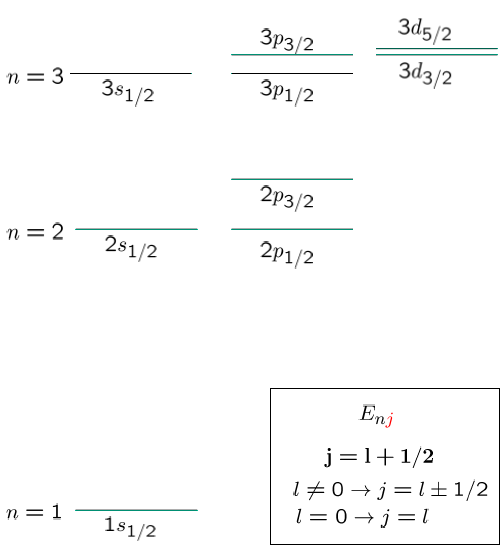
\includegraphics[scale=0.45]{ch1/image82}
	\captionof{figure}{ }
	\end{wrapfigure}
	
Sans surprise, l'énergie de \textsc{Dirac} dépend de $n$, mais aussi du nombre quantique $j$
\begin{equation}
E_{nj}^D = mc^2\times \left[ 1 + 
\left(
\frac{Z \alpha} {n-j-1/2 + [(j+1/2)^2 - Z^2 \alpha^2)^{1/2}}
\right) ^2  \right] ^{-1/2}
\end{equation}
Il s'agit de la solution analytique de \textsc{Dirac}. Afin de faire le lien avec 
\textsc{Schrödinger}, nous allons étudier le comportement de cette solution lorsque $Z\alpha$ n'est
pas trop important ou, autrement dit, lorsque les effets relativistes ne sont pas trop grands. 
Développons alors en puissance de $(Z\alpha)^2$
\begin{equation}
E_{nj}^D = mc^2= mc^2 \left[
1 - \frac{(Z \alpha)^2}{2 n^2} 
- \frac{(Z \alpha)^4}{2n^4} \left(
\frac{n}{j+1/2} - \frac{3}{4} \right) + \ldots \right]
\end{equation}\ \\
Bonne nouvelle : l'énergie relativiste de \textsc{Dirac} n'est autre que $mc^2$ et si on retire cette
énergie, il y a toujours une dépendance en $n$ et $j$. Il est donc possible d'exprimer, en faisant
cette soustraction, l'énergie non relativiste à laquelle s'ajoute des corrections proportionnelles
à l'énergie relativiste\footnote{Pour rappel, le solutions de l'équation de Schrödinger sont 
données par $E_n^{\mbox{NR}} =
- \frac{1}{2} \mu c^2 \frac{(Z \alpha)^2}{n^2} ; \hspace*{1cm}
{\color{red} \alpha = \frac{e^2}{(4 \pi \epsilon_0) 
\hbar c}}$.}
\begin{equation}
E_{n {\color{red} j}} = E^D_{nj} - mc^2 = E_n^{\mbox{NR}} \left[
1 + \frac{(Z \alpha)^2}{n^2} \left(
\frac{n}{{\color{red} j}+1/2} - \frac{3}{4} \right) + \ldots \right]
\end{equation}
Les corrections dépendent évidemment de $j$ et c'est rassurant car si $c\to \infty$, on retrouve
l'énergie non-relativiste qui n'est autre que la valeur propre de l'équation de \textsc{Schrödinger}.


\subsection{Fonctions radiales de Dirac}
Représentons l'orbitale $R$ de \textsc{Dirac}. Soit l'atome de $Hg^{79+}$ où 79 électrons ont été
arrachés de façon à former un système hydrogénoïde. En rouge, la \textit{grande composante} $P$ 
rappelle l'orbitale $2s$. On comprend également la désignation \textit{petite composante} à l'aide
de la courbe en vert représentant $Q$. Si $c\to\infty, Q\to 0$ et la petite composante s'éteint : on
retrouve l'expression de $P$ identique à celle trouvée avec \textsc{Schrödinger}. On peut remarquer
que ces deux composantes ne s'annulent pas au même rayon $r$. La somme des deux composantes ne 
s'annulera donc jamais : disparition de la structure noeudale.\\


On peut voir que l'effet non-relativiste n'est pas négligeable lorsque l'on représente la densité
$NR$ de \textsc{Schrödinger} $D_{n l}(r) = \vert P_{nl}(r) \vert^2 = r^2 R_{nl}(r) ^2$ et la 
densité $R$ de \textsc{Dirac} $D_{n \kappa}(r) = \vert P_{n \kappa}(r) \vert^2
+  \vert Q_{n \kappa}(r) \vert^2$.\\

Comme prévu, la densité ne s'annule jamais. On observe également une contraction de l'onde signifiant
une contraction de l'énergie de liaison. La structure ressemble cependant toujours à celle de 
\textsc{Schrödinger}. Cet effet est également présent dans d'autres orbitales (voir \textit{slide 
45}).


\begin{center}
	\includegraphics[scale=0.4]{ch1/image9}
	\captionof{figure}{ }
\end{center}

\newpage
\subsection{Limite non relativiste de Dirac}
Il n'est pas possible d'ignorer les résultats obtenu par l'équation de \textsc{Dirac}. Cependant, 
il est possible d'essayer de "mimiquer" le spectre de \textsc{Dirac} en bye-passant la complexité
de son équation. L'idée est d'exprimer l'Hamiltonien de Dirac comme un de Schrödinger additionné à
une perturbation de sorte à pouvoir écrire $H \psi ({\bf r}) = E' \psi ({\bf r})$. \\

Les corrections proposées ci-dessous vont être correctes jusqu'à l'ordre $(v/c)^2$. Considérons un
potentiel central
\begin{equation}
\left\{
\begin{array}{l}
{\bf A } = 0 \\
q \Phi = - e \Phi = V(r) = -\frac{Ze^2}{(4 \pi \epsilon_0) r}
\end{array} \right.
\end{equation}
En mimiquant, on obtient
\begin{equation}
H = \frac{p^2}{2m} + V(r)- \frac{p^4}{8 m^3 {\color{red} c^2}} 
+ \frac{1}{2m^2 {\color{red} c^2}} \frac{1}{r}
  \frac{dV}{dr} {\bf L} \cdot {\bf S} 
 + \frac{\pi \hbar^2}{2 m^2 {\color{red} c^2 } }
  \left( \frac{Ze^2}{4 \pi \epsilon_0} \right) \delta( {\bf r} )
\end{equation}
où $V(r)$ est le potentiel d'interaction des protons, où l'on retruve une correction de \textit{masse
à l'énergie cinétique}
\begin{equation}
H^{\mbox{M}} = - \frac{p^4}{8 m^3 c^2}
\end{equation}
Une correction due à l'interaction \textit{spin-orbite}
\begin{equation}
H^{\mbox{s-o}} = + \frac{1}{2m^2 c^2} \frac{1}{r}
  \frac{dV}{dr} {\bf L} \cdot {\bf S} 
\end{equation}
Et une correction de \textit{Darwin}
\begin{equation}
H^{\mbox{D}} = 
 + \frac{\pi \hbar^2}{2 m^2 c^2 } 
  \left( \frac{Ze^2}{4 \pi \epsilon_0} \right) \delta( {\bf r} )
\end{equation}

La correction la plus parlante est l'interaction spin-orbite venant du fait que \textsc{Dirac} a 
forcé le couplage entre $\vec{L}$ et $\vec S$. Les deux autres corrections sont assez difficile à 
interpréter physiquement et il n'existe pas de consensus sur leur interprétation, nous n'y reviendrons
pas. Notons la signature relativiste de ces corrections via le facteur $1/c^2$. Le \textit{slide 47}
montre l'impact de ces différents corrections au sein de la couche $n=2$. Les \textit{slides 48} à
\textit{53} seront vus en séance d'exercices et ne sont pas repris ici (le but est de dériver
l'expression de l'énergie dû à la structure fine)\footnote{Lire notes personnelles \textit{slide 54}}.



\newpage
\section{Lamb shift (1947)}
\subsection{Levée de la dégénérescence pour $j=1/2$}
La catastrophe (ou beauté) c'est que tout n'est pas prévu par l'équation de \textsc{Dirac}. En 
observant les niveaux $n=2$, \textsc{Lamb} a obtenu trois niveaux et non pas deux comme le 
prévoyait\textsc{Dirac} : il y a une levée de la dégénérescence pour $j=1/2$.\\

	\begin{wrapfigure}[9]{l}{6cm}
	\vspace{-5mm}
	\includegraphics[scale=0.4]{ch1/image10}
	\captionof{figure}{ }
	\end{wrapfigure}
L'énergie dépend non seulement de $j$, mais peut-être bien de $n$ également. Il s'agit d'un effet 
plus fin que la structure fine, mais ce n'est pas la structure \textit{hyperfine} non plus. Il 
s'agit de la première manifestation pour un électron de l'électrodynamique quantique. Cet effet
est causé par les oscillations du vide\footnote{Si l'on admet que le vide sont des petits OH, on 
est forcée de constater que même à température nulle le système vibre encore ($E_v = \hbar\omega/2$.
Il existe donc un champ électromagnétique oscillant dans le fondamental que l'on nomme 
\textit{oscillation du vide du champ EM}.} que \textsc{Dirac} ne prend pas en compte. Or, un 
électron $2s$ ressent ces oscillation différemment qu'un électron $2p$ mais pour calculer ces 
déplacements, il faut se tapper un diagramme de \textsc{Feynman}.\\

L'énergie d'ionisation de l'hydrogène est d'à peu près 110 000 cm$^{-1}$. Ce déplacement de 
\textsc{Lamb} est d'à peu près 0.038 cm$^{-1}$ pour l'hydrogène mais peut atteindre 75 eV pour 
l'uranium.


\section{Structure hyperfine de l'hydrogène}
	\begin{wrapfigure}[14]{r}{7cm}
	\vspace{-5mm}
	\includegraphics[scale=0.5]{ch1/image11}
	\captionof{figure}{ }
	\end{wrapfigure}
On s'intéresse ici à un effet nucléaire sur la structure électronique. Avec une résolution 
suffisamment fine, on s'aperçoit qu'il n'y a pas deux niveau pour $n=1$ mais quatre. Regardons
l'état fondamental $1s$ en Schrödinger qui devient $^2S_{1/2}$ dans Dirac\footnote{Le 2 en haut à 
gauche représente un \textit{doublet} car l'électron peut être dans deux états de spin (
$S=1/2, m_s =\pm1/2$ : \textit{up} et \textit{down}. Lorsque $S=1, m_s=-1,0,1$ et on parle de triplet.
De même lorsque $S=3/2$, $m_s = \pm 1/2, \pm 3/2$ et on parle de quadruplet, etc. }. \\

Cet effet s'observe même dans un cage de \textsc{Faraday} isolé de tout champ. Cependant, lorsque
l'on place un champ d'induction magnétique le niveau (pour $n=1$) $F=0$ donne un niveau tandis que
$F=1$ se divise en trois niveau (levée de dégénérescence). Il faut trouver quelque chose qui 
préserve l'invariance par rotation mais donnant un couplage\footnote{Si $F=2$, nous aurons 5 
valeurs.}. \\

Ce quelque chose c'est le noyau car le proton ($^1$H) possède un moment angulaire ; un spin noté
$I=1/2$. Il va y avoir un couplage entre $J$ (nature électronique) et $I$ (nature nucléaire)
\begin{equation}
{\bf F} = {\bf J} + {\bf I} \Rightarrow 
F = J+I, J+I-1, \ldots, \vert J-I \vert
\end{equation}
Notons que la théorie de l'électrodynamique quantique justifie un déplacement du fondamental mais
ne met pas en évidence un nouvelle structure. Cette dernière apparaît cependant bien lorsque
l'on \textit{regarde de plus près}. Remarque : $1GHz$ correspond à $\pm 10^{-6}$ eV ce qui n'est 
pas grand chose!\\

Pour chiffrer ces effets, on utilise le \textit{moment magnétique de spin $\mu_I$}, le 
\textit{magnéton de Bohr} $\mu_B$ et le \textit{magnéton nucléaire} $\mu_N$
\begin{equation}
\mbox{\boldmath $ \mu $}_I = g_I \mu_N {\bf I}/ \hbar,\qquad\qquad
\mu_B = \frac{e \hbar}{2m_e},\qquad\qquad
\mu_N = \frac{e \hbar}{2M_p} = \frac{m_e}{M_p} \mu_B
\end{equation}
Le moment nucléaire est colinéaire au moment magnétique : le rapport $\mu_N/\mu_B$ vaut à peu près
1836. La définition de $\vec F$ crée évidemment un nouvel \textsc{ecoc}.

\subsection{État fondamental $1s_{1/2}$}
Considérons l'interaction hyperfine dipolaire magnétique (M1)
\begin{equation}
H = H^0 + H^{M1}
\end{equation}
Il existe des interactions avec le spin de l'électron. Dans l'état $1s$, nous avons 
${\bf J} = {\bf L} + {\bf S} = {\bf S}$. En définissant $\mbox{\boldmath $ \mu $}_S = -g_S \mu_B {\bf
S}/ \hbar$, on peut écrire un Hamiltonien décrivant cette interaction
\begin{equation}
H^{M1}_{\mbox{spin}} = - \mbox{\boldmath $ \mu $}_S \cdot 
{\bf B} = 2 \mu_B {\bf S} \cdot {\bf B} / \hbar
\end{equation}
Pour l'obtenir on travaillera avec le potentiel vecteur ${\bf A} ({\bf r}) = - \frac{\mu_0}{4 \pi}
\left[ \mbox{\boldmath $ \mu $}_I \times \mbox{\boldmath $ \nabla $} \left( \frac{1}{r} \right)
\right]$ avec lequel il est possible d'en tirer ${\bf B} = \mbox{\boldmath $ \nabla $} \times {\bf A}
= -\frac{\mu_0}{4 \pi} \left[\mbox{\boldmath $ \mu $}_I \nabla^2 \left( \frac{1}{r}  \right)
 - \mbox{\boldmath $ \nabla $} ( \mbox{\boldmath $ \mu $}_I \cdot \mbox{\boldmath $ \nabla $} )
\frac{1}{r} \right]$. Malheureusement, nous n'avons pas le temps de nous attarder la dessus.\\

Notons cependant que via l'\textit{interaction de contact de Fermi} ($m=0$), nous pouvons écrire
que
\begin{equation}
\nabla^2 \left( \frac{1}{r} \right)  
= -4 \pi {\color{red} \delta ({\bf r})  } \neq 0 
\hspace*{1cm}
{\color{red} ~\mbox{ssi}~l=0  }
\hspace*{1cm} (R_{nl} (r) \sim r^l )
\end{equation}
Il s'agit de l'équation de \textsc{Poisson}.On peut ré-écrire notre Hamiltonien
\begin{equation}
H^{M1}_{\mbox{spin}}  =  
\frac{\mu_0}{4 \pi} \frac{2}{\hbar^2} 
g_I \mu_B \mu_N 
\frac{8 \pi}{3} 
{\color{red}  \delta( {\bf r})}
\;  {\bf S} \cdot {\bf I}
\end{equation}
On peut lier cette relation avec la correction de \textsc{Darwin} qui contenait un $\delta(\vec{r})$,
il s'agit d'une première justification de cette expression.


\subsection{État $ns_{1/2}$}
Nous avons précédemment établi 
\begin{equation}
H^{M1}_{\mbox{spin}}  =  \frac{\mu_0}{4 \pi} \frac{2}{\hbar^2} g_I \mu_B \mu_N \frac{8 \pi}{3} \delta( {\bf r})
\;  {\bf S} \cdot {\bf I}
\end{equation}
Dans notre cas $l = 0 \Rightarrow {\bf F} = {\bf J} + {\bf I} =  {\bf S} + {\bf I}$ et donc 
${\bf S} \cdot {\bf I} = \frac{1}{2} ({\bf F}^2 - {\bf I}^2 - {\bf S}^2)$.\\

Nous pouvons écrire le \textit{ket} suivant, où nous avons couplé $S$ et $I$ pour donner $F$
\begin{equation}
\vert ns_{1/2}IFM_F \rangle=  \sum_{(m_j=m_s),M_I}
\vert ns_{1/2}m_s I M_I \rangle 
\langle ns_{1/2}m_s I M_I 
\vert ns_{1/2}IFM_F \rangle  
\end{equation}
Ce qui nous permet de calculer l'énergie moyenne
\begin{equation}
\Delta E_{\color{red} F} = \langle ns_{1/2}IFM_F \vert H^{M1}_{\mbox{spin}}
\vert ns_{1/2}IFM_F \rangle  = \frac{A}{2} [ {\color{red} F}({\color{red} F}+1) 
- I(I+1) - \frac{1}{2}(\frac{1}{2}+1)]
\end{equation}
où $\DS A =
\frac{\mu_0}{4 \pi} 2  
g_I \mu_B \mu_N \frac{8 \pi}{3} 
 {\color{red} \langle \delta( {\bf r})  \rangle }$. Calculons la valeur moyenne du delta de
\textsc{Dirac}
\begin{equation}
\langle \delta( {\bf r}) \rangle = \int \vert \psi_{n00} (r) \vert^2
\delta( {\bf r} ) d{\bf r} = \vert \psi_{n00} (0) \vert^2 = 
\frac{{\color{red} Z^3}}{\pi a_\mu^3 {\color{red} n^3}}
\end{equation}
Cette valeur moyenne n'est pas nulle grâce à faut qu'il n'y a pas d'annulation en $r=0$ pour les
électrons $s$. On en tire
\begin{equation}
A =
\frac{\mu_0}{4 \pi}  \frac{16 \pi}{3} g_I \mu_B \mu_N  
\frac{Z^3}{\pi a_\mu^3 n^3}
\end{equation}


\subsection{Levée de dégénérescence pour $1s_{1/2}$}
Une image vaut mieux qu'un long discours

\begin{center}
\includegraphics[scale=0.45]{ch1/image12}
\captionof{figure}{Notons pour le $^1$H le bon accord théorie expérience : $v_{th} \approx 1420$ MHz, 
$\nu_{exp} = 1420405751.800$ Hz. Il s'agit de la raie à $\lambda=21$ cm.}
\end{center}






\subsection{Interaction hyperfine électrique quadrupolaire}
En plus de l'interaction hyperfine dipolaire magnétique $M1$ dont nous avons discuté ci-dessus, il
existe l'interaction hyperfine électrique quadrupolaire $E2$\footnote{Voir cours de \textit{Physique
nucléaire.}}
\begin{equation}
H = H^0 + H^{M1} + H^{E2}
\end{equation}
Nous avions déjà énoncé le moment magnétique de spin $\mbox{\boldmath $ \mu $}_I = g_I \mu_N {\bf I}/
\hbar$. Définissons maintenant le \textit{moment quadrupolaire électrique du noyau}
\begin{equation}
Q = \langle I, M_I=I \vert Q_{zz} \vert I, M_I=I \rangle
= \langle I, M_I=I \vert \sum_p (3 z^2_p - r^2_p)  \vert I, M_I=I \rangle
\end{equation}
Si l'on effectue le changement de variable $z=r\cos\theta$, on retrouve la partie radiale de 
$Y_{20}$. La valeur moyenne de ce moment angulaire se calcule alors
\begin{equation}
Q_{20} = sum_p r_p^2 Y_{20}(\Omega_p)
\end{equation}
où l'on somme sur tous les protons\footnote{Il faudrait expliciter, je n'ai pas tout compris. Il 
faut les notes du tableau!}. La composante $z$ peut être calculée par deux fonctions
nucléaires. En fonction du signe de $Q$ trois cas peuvent se présenter (soit la distance de charge 
nucléaire) : sphérique $(Q=0)$, prolate ($Q>0$) et oblate ($Q<0$). Si $I=0$ ou $I=1/2$, il en vient
que $Q=0$. Par exemple, $Q(^2\mbox{H}) = 0.0028~\mbox{barns} = 0.0028~10^{-24}~\mbox{cm}^{2}$.



\section{Largeurs de raies}
\subsection{Largeur naturelle}

	\begin{wrapfigure}[15]{r}{5cm}
	\vspace{-5mm}
	\includegraphics[scale=0.5]{ch1/image13}
	\captionof{figure}{ }
	\end{wrapfigure}
	
Même si \textsc{Schrödinger}, \textsc{Dirac}, \dots prévoient tous des niveaux bien distincts, ce 
n'est pas le cas en pratique (à cause des incertitudes sur les niveaux). Il peut donc pour une 
transition entre deux niveau, émettre des photons de différentes énergies (à cause des incertitudes
sur les deux niveaux). On peut montrer que la largeur naturelle (qui concerne même le fondamental et
qui donc empêche d'avoir des raies parfaitement piquées) est un profil lorentzien, ici exprimé 
en fonction de l'intensité
\begin{equation}
I(\nu) = I_0 \; \frac{ (\gamma / 4\pi )^2}
{ (\nu - \nu_0 )^2 + (\gamma / 4\pi )^2 }
\end{equation}
On peut en définir la largeur à mi-hauteur $\delta \nu_L = \gamma / 2 \pi$. Ce coefficient $\gamma$
n'est en réalité rien d'autre que le coefficient d'\textsc{Einstein} d'émission spontanée
\begin{equation}
\gamma = A_{21} = 1 / \tau_2 \rightarrow 
\delta \nu_L = \frac{1}{2 \pi \tau_2}
\end{equation}
ici de $2\to1$. Comme mentionné ci-dessus, il faut tenir compte de l'incertitude des deux niveaux. 
La largeur à mi-hauteur s'écrit alors
\begin{equation}
\delta\nu_{12}=\delta\nu_1+\delta\nu_2 = \frac{1}{2\pi}\left(\frac{1}{2\pi\tau_2}+\frac{1}{2\pi\tau_2}
\right)
\end{equation}



\subsection{Élargissement par pression}
Comme on l'a déjà dit, même avec \textsc{Dirac, Schrödinger}, \dots où on croit avoir une raie bien
pure il y aura un élargissement, notamment par pression. La forme mathématique est équivalente, il
s'agit d'une lorentzienne
\begin{equation}
I(\nu) = I_0 \; \frac{ (w/2 )^2}
{ (\nu - \nu_0 - d )^2 + (w/2 )^2 }
\end{equation}
Sauf qu'ici, la largeur à mi-hauteur est liée à $w$ qui vaut
\begin{equation}
w =  \frac{1}{ 2 \pi t_0}
\end{equation}
où l'on voit apparaître $t_0$, le temps moyen entre collisions. A pression nulle, chaque particule 
possède un libre parcours moyen infini. Pour se débarrasser de cet effet on effectue les manipulations
à différentes mesures et on essaye d'extrapoler à pression nulle afin d'avoir un signal "idéal". Les
manipulations d'atomes froids sont aussi courants dans ce domaine.


\subsection{Élargissement Doppler}
Hélas il n'y avait pas que cet effet et il y a bien pire : l'effet \textsc{Doppler}
\begin{equation}
\omega = \left(
\frac{1 \mp v/c}{1 \pm v/c} \right) ^{1/2} \omega_0
\end{equation}
La fréquence que l'on voit dans une raie n'est propre que s'il n'y a pas ni mouvement, ni dynamique
entre la source émettrice et l'observateur (ou l'inverse). La fréquence apparente n'est pas la 
fréquence propre. Développons en série
\begin{equation}
\omega - \omega_0 = \mp \frac{v}{c} \omega_0
+ \frac{1}{2} \frac{v^2}{c^2} \omega_0 + \ldots
\end{equation}
Au premier ordre
\begin{equation}
\omega = \omega_0 \left( 1 \mp \frac{v}{c} \right),\qquad\qquad\qquad
\lambda = \lambda_0 \left( 1 \pm \frac{v}{c} \right)
\end{equation}
On peut alors avoir un \textit{red-shift} $\omega = \omega_0 \left( 1 {\color{red} - } 
\frac{v}{c} \right)$ ou un \textit{blue-shift} $\omega = \omega_0 \left( 1 {\color{blue} + } 
\frac{v}{c} \right)$.\\

C'est lorsque une source d'émission s'approchant de l'observateur à vitesse $v_x$ que l'on parle
de décalage vers le bleu. Celui-ci est donné par
\begin{equation}
- \frac{\Delta \lambda }{\lambda_0} =
\frac{\Delta \nu}{\nu_0} = \frac{ \nu - \nu_0 }{\nu_0}  
= \frac{v_x}{c}
\end{equation}
La distribution de Maxwell des vitesses des atomes nous permet, à l'équilibre et à la température
$T$, de connaître la fraction d'atomes ayant une vitesses comprises entre $v_x$ et $v_x+dv_x$
\begin{equation}
dN(v_x) = N_0 \exp (-M v_x^2 /2kT) \; dv_x
\end{equation}
Avoir connaissance de la vitesse est important : l'effet \textsc{Doppler} est nul pour une source 
se déplaçant orthogonalement à l'observateur, mais est colossal lorsqu'une particule se rapproche
vers l'observateur.\\

La profil est cette fois-ci gaussien
\begin{equation}
I(\nu) =  I_0 \; e^{-x^2}~~\mbox{avec}~~
x = 2 \sqrt{\ln 2} \; \frac{\nu_0 - \nu}{\delta \nu_D}
\end{equation}
La largeur à mi-hauteur (\textsc{fwhm}) est donnée par
\begin{equation}
\delta \nu_D = 
2 \sqrt{\ln 2} \; \frac{\nu_0}{c} 
 \sqrt {\frac{2 k{\color{red} T}}
{ {\color{red} M} }}
\end{equation}
Cette largeur est inversement proportionnelle à la racine de la masse. Si la masse est grande, pour
une même énergie, la particule ne se déplacera pas de la même façon. La largeur \textsc{Doppler} sera
donc suffisamment mince pour de gros noyaux. On s'intéresse ici également aux atomes froid, dont le
but est d'immobiliser un atome. S'il est piéger, il ne subit plus d'effet de pression et il n'y a 
pas d'effet \textsc{Doppler}.\\

	\begin{wrapfigure}[8]{r}{5.7cm}
	\vspace{-5mm}
	\includegraphics[scale=0.4]{ch1/image14}
	\captionof{figure}{ }
	\end{wrapfigure}
Cet effet peut paraître anodin, mais on l'a rencontré dans l'étude
des systèmes binaires (décale une raie parfois dans un sens, parfois dans l'autre). Autre exemple,
\textsc{Ewen} et \textsc{Purcell} n'ont pas observé une raie bien étroite de 21cm en observant la
\textit{Milkyway}, mais une raie avec une certaine largeur. En pointant sur le centre de la 
galaxie, certaines étoiles se rapprochent et d'autres s'éloignent : shift. C'est ce qui a permis de
modéliser la forme de notre galaxie.


\subsection{Comparaison des profils Doppler et Lorentzien, convolution et profil de Voigt}
Lorsque les deux effets sont présents en même temps, il se produit une convolution entre ces deux effets. Ceci donne un \textit{profil de} \textsc{Voigt}
\begin{equation}
I(x) = \mbox{cste} \; 
\int_{-\infty}^\infty 
\frac{e^{-y^2}}{(x-y)^2 + a^2} dy
\end{equation}
où $\DS x = 2 \sqrt{ \ln 2} \; \;
\frac{\nu_0 - \nu}{\delta \nu_D}$ et $\DS a =  \sqrt{ \ln 2} \; \; 
\frac{\delta \nu_L}{\delta \nu_D}$.

\chapter{Centrifugal pumps}
\section{Generalities}
\subsection{Description - Type of turbopump}
\minifig{ch2/1}{ch2/2}{0.3}{0.4}{0.2}{0.3}
The task of the turbopump is to transfer energy to a liquid. Above we can see a centrifugal and an axial turbopump. Between these two extremes, we can have a variety of of types depending on the requirements. Each turbopump is composed of one or several wheels that can be mounted in parallel (increase mass flow rate) or in series (higher energy transfer), see \autoref{ch1/2}. 

\subsection{Installation of a turbopump}
\minifig{ch2/3}{ch2/4}{0.3}{0.25}{0.2}{0.3}
The general scheme is shown here, observe that the flow enters at the middle in the rotating blade and is projected into the volute. This last has a growing section from the beginning to the end as the mass flow increases. The turbopump is commonly used to transfer liquid from a downstream reservoir to an upstream reservoir situated higher. We have to be careful to avoid cavitation (evaporation of the fluid due to too low pressures) and we also have a control valve at the suction section to always have a contact blade-fluid.

\subsection{Energy developed by the turbopump - flow rate}
\wrapfig{8}{l}{4.5}{0.2}{ch2/5} 
This is the type of curve we will have with the equations, where we see the characteristic curves of the pump and of the overall system (model of the resistance). These curves will be very similar to compressors. Depending on the rpm, we will consider different curves. The fundamental equations are simplified considering $\rho = cst \rightarrow \nu = cst$ for non compressible fluids: 

\begin{equation}
e = \frac{v_o^2 - v_i^2}{2} + \int _{p_i}^{p_o} \nu dp + g(h_o - h_i) = \frac{v_o^2 - v_i^2}{2} + \frac{p_o-p_i}{\rho} + g(h_o - h_i)
\end{equation}

The velocity is low in order to limit the head losses and thus the pressure term is the highest (height change in a compressor is low too). The energy delivered by the pump to the fluid can be rewritten in terms of the volumetric flow rate $Q$ [$m^3/s$]: 

\begin{equation}
e_p = \frac{p_a - p_i}{\rho} - \frac{p_a - p_o}{\rho} + \frac{A_i^2-A_o^2}{2A_iA_o}Q^2 + g(z_o-z_i)
\end{equation}

\subsection{Useful power or hydraulic power}
The power transfered from the input of the pump until the exit and the global efficiency of the pump are: 

\begin{equation}
P_h  = \dot{m}e = \rho Q e \quad [W] \qquad \eta = \frac{\rho Q e}{P_m}
\end{equation}

where $P_m$ is the mechanical power to drive the pump. 

\subsection{Working point of a turbopump}
Consider \autoref{ch2/4} and let's apply Bernouilli equation (kinetic energy equation) between $z'$ and $z_i$ then $z_o$ and $z^"$: 

\begin{equation}
\frac{v_i^2 - {v'}^2}{2} + g(z_i - z') = -\frac{p_i - p'}{\rho} -w'_{fa} \\ \frac{{v^"}^2 - {v_o}^2}{2} + g(z^" - z_o) = -\frac{p^" - p_o}{\rho} -w'_{fr}
\end{equation}

One can make the sum of the two expression and regroup the terms of the reservoirs in a new \textbf{energy requested by the circuit} $\bm{e_n}$. If we consider large reservoirs $v^" \approx v'$ and $p^"\approx p' \approx p_a$, we have: 

\begin{equation}
e_n = g(z^"-z') + \underbrace{w'_{fa} + w'_{fr}}_{w'_f} \qquad \Rightarrow e_p = e_n 
\end{equation}

This is always valid in \textbf{steady state}. 

\subsection{Characteristic of the hydraulic circuit}
The system curves on \autoref{ch2/5} plot $e_n$ which depends on the height difference and the mass flow rate (because $w'_f\propto v^2$ of the flow) and depends thus on the square of the volumetric mass flow rate. This is why we have a parabolic shape, the slope depends on the head loss coefficient $K$. If we have a valve, the closer the valve, the higher the slope. 

\subsection{Performance curve of a pump}
Similar curves can be established for the $e, Q$ relations at different rpm. With a control valve at the exit, and by fixing the rpm of the engine, we can find them and are plotted on \autoref{ch2/5}. 

\subsection{Working regimes}
Practical analysis shows that if two of the three parameters $e,Q,n$ are fixed, the working point too: $f(e,Q,n) = 0$

\subsection{Practical units}
\wrapfig{8}{l}{5}{0.45}{ch2/6}
Here we express the energy in $J/kg$ but we know that it is also $g\Delta z$ in [m]. Thus we will use instead of $e$, $H = e/g$ [m]. The energy transferred to the fluid is often called the \textbf{height} of the \textbf{head}. For example $H = 10$ m means that we transfer energy such that we increase $z$ of 10 m. As last remark, be aware that efficiency curves are provided by the manufacturer and the pump has to be chosen specifically to the circuit where it should operate to get the maximum efficiency. 

\section{The centrifugal pump}
\subsection{Organization of a centrifugal pump}
\wrapfig{8}{r}{4}{0.3}{ch2/7}
We have an inlet distributor D charged of guiding the fluid towards the entrance 1 of the rotor R or also called \textbf{impeller}. The rotor is made of one or two disks on which are mounted the blades beginning at a certain external radius $r_1$ and finishing at $r_2$. A fixed diffuser d composed of 2 parallel discs surrounding the rotor, connected with vanes surrounds the exit of the blades, sometimes it is not used. A \textbf{volute} or \textbf{collector} c with increasing volume directs the flow to the exit section of the machine. 

\subsection{The distributor}
If there is no vane in the distributor, the flow penetrates in the rotor axially since we assume no fluid particle to rotate before entering in the rotor, and becomes radial symmetrically at intrance 1. If there is vane, the direction of the flow is imposed by the vanes but we take the first case here. The equation of kinetic energy applied between i and 1 when neglecting the height difference is: 

\begin{equation}
\frac{v_i^2-v_1^2}{2} + \frac{p_i-p_1}{\rho} = w'_{fD}
\end{equation}

where $w'_{fD}$ represents the pressure losses in the distributor, proportional to the square of $Q$ and thus to $v_1^2$: $w'_{fD}= K_D \frac{v^2_1}{2}$ where $K_D \approx 5.10^{-3}$

\subsection{The rotor}
The impeller starts at $r_1$ and finish at $r_2$, the section of the rotor at these levels are: 

\begin{equation}
A_1 = 2\pi r_1b_1 e_1 \qquad A_1 = 2\pi r_2b_2 e_2
\end{equation}

where $e_1,e_2$ are blockage coefficients taking into account the decrease in area due to the thickness of the impeller. 

\wrapfig{12}{l}{4.5}{0.3}{ch2/8}
The rotor and impeller velocity triangles are represented on the figure. $v_1$ is known by the previous discussion and is purely radial and $u_1$ can be computed: 

\begin{equation}
v_1 = \frac{Q_R}{2\pi r_1 b_1 e_1} \qquad u_1 =r_1\omega _1 = \frac{2\pi n}{60} r_1 \qquad \alpha _1 = 90\degres
\end{equation}

The missing components of the velocity triangles are $w_1$ and $\beta _1$ and can be retrieved by construction. In addition we make an assumption for $\beta _1$ (fluid angle) which must be equal to $\bar{\beta} _1$ (solid angle), this is imposed by the design to avoid collision or separation. Indeed, the pump is designed to work with a certain $Q_R$ and a certain $n$, if this changes, shocks and separation can occur, leading to losses. Same considered for $\beta _2$, $u_2 = r_2 \omega$ and this time the radial velocity is the projection of $w_2$: 

\begin{equation}
u_2 = r_2 \omega _2 \qquad w_2 \sin \beta _2 = \frac{Q_R}{2\pi r_2 b_2 e_2}
\label{2.9}
\end{equation}

$\beta _2$ is chosen larger than 90\degres in order to make $v_2$ small and thus limit the diffuser size (limit the losses, $\beta _2$ between 145\degres and 165\degres). We are now able to retrieve $v_2$ and $w_2$. 

\subsection{Number and shape of the blades}
\wrapfig{10}{r}{5}{0.3}{ch2/9}
The number of blades determine the volume available to the flow and the guidance. The more we have blades, the more the fluid is guided but the more we have pressure losses. The designer must make a trade-off, generally there are 6 to 12 blades. The profile of the blades must be so that the angles $\beta _1 = \bar{\beta}_1$ and $\beta _2 = \bar{\beta}_2$ are respected. 

\ \\
If the blades are made of two surfaces, one active and one non-active as represented on the figure, if the the two surfaces makes an angle too large at the entrance, it is impossible that $\beta _1$ is tangent to both and lead to shocks. At the exit, since there is a pressure gradient between active and non active sides, the $\beta _2$ is "sucked" by the non-active part where the pressure is lower. 

\subsection{Head of Euler of the rotor}
Using Euler-Rateau and power distribution, we have: 

\begin{equation}
P_R =  \dot{m}_R (u_2v_{2u}-u_1v_{1u}) = \dot{m}_R e_R + \dot{m}_R w^"_{fR} \qquad \Rightarrow e_R = u_2v_{2u}-u_1v_{1u} - w^"_{fR}
\end{equation}

\wrapfig{5}{l}{4}{0.25}{ch2/10}
as we have seen, $\alpha _1 = 90\degres \Rightarrow v_{1u} = 0$ and $e_R = u_2v_{2u} - w^"_f$. The term $u_2v_{2u}$ is called the \textbf{energy of Euler} and is the theoretical energy that the rotor transfers to the fluid. The \textbf{head of Euler} is $\frac{u_2v_{2u}}{g}$. Lets show that this energy is function of $Q_R, N, \bar{\beta}_1$ and $\bar{\beta _2}$ using the velocity triangle relation: 

\begin{equation}
\bm{u_2} v_2 \cos \alpha 2 = \bm{u_2}  (u_2 + w_2 \cos \bar{\beta} _2) \Rightarrow e_r = u^2_2 + \frac{Q_R}{2\pi r_2 e_2 b_2 \tan \bar{\beta} _2}
\end{equation}

where we used \autoref{2.9}. We see that as $\bar{\beta}_2>90\degres$ in practice, we have a linearly decreasing function. We still don't have the characteristics since we are underestimating the angles deviation, the number of blades and the fluid losses. 

\subsection{Losses in the rotor due to friction}
He skipped the previous section. The term $w^"_f$ regroups the different losses that occurs in the rotor and can be separated in:\\ 

\begin{itemize}
\item[•] the losses due to the development of the boundary layer in the channel sidewalls and $\propto Q_R^2$: 

\begin{equation}
k_1 Q_R^2 = K_R\frac{w_1^2}{2} \qquad K_R \approx 0.025
\end{equation}

\item[•] a second loss due to the shocks and separation of the boundary layer each time $w_2$ is not tangent to the blade. Looking to the situation on \autoref{ch2/11}, we find experimentally that these losses are $\propto (\Delta w)^2$ that is $\propto v_1$ that is $\propto Q_R - Q_{RD}$ where $Q_{RD}$ is the flow rate in design conditions $\beta _1 = \bar{\beta} _1$: 

\begin{equation}
Q_R = 2\pi r_1 b_1 e_1 v_1 \qquad Q_{RD} = 2\pi r_1 b_1 e_1 v_{1D}
\end{equation}  
\end{itemize}

\minifig{ch2/11}{ch2/12}{0.3}{0.28}{0.3}{0.3}

The sum is represented on \autoref{ch2/12} and we see that even at low $Q_R$ $w^"_f$ is high, this is due to the second loss. 

\subsection{Loss due to the internal leak flow}
We already know what it is, it goes from 1 for large pumps to 10\% of $\dot{m}_R$ for small pumps. This is due to the fact that the clearance cannot be reduced under an absolute size and the seals in large machines cannot be more efficient than in small machines. The power loss is: 

\begin{equation}
\dot{m}_i e_R = (0.01\ to\ 0.1)\dot{m}_Re_R \quad [W]
\end{equation}

\subsection{Friction of the disc on the non-active fluid}
Per side of the disc, it can be estimated as: 

\begin{equation}
P_{fr} = 1.21 \, 10^{-3} u_2^3 D_2^2 \quad [ch]
\end{equation}

\subsection{The diffuser}
\subsubsection{Energy transformation in the diffuser}
The velocity $v_2$ at the exit of the pump is generally too high for some applications, the diffuser converts part of the kinetic energy into pressure energy. There exists 4 types of diffuser: straight parallel sidewalls or inclined, and for each we can have vaned or vaneless. The kinetic energy equation in a fixed frame with $z_3 - z_2 = 0$ is: 

\begin{equation}
\frac{p_3-p_2}{\rho} = -\frac{v_3^2-v_2^2}{2} -w'_{fd}
\end{equation}

where $w'_{fd}\approx 0.02 - 0.03 v^2_2/2$ [J/kg]. We see that kinetic energy gives pressure and loss. 

\subsubsection{The vaneless diffuser with flanges} 
\wrapfig{10}{l}{4}{0.4}{ch2/13}
The common architecture of the diffuser is composed of two circular flanges put around and in the continuity of the exhaust of the rotor. Let's apply the equation of the kinetic moment to a fluid element of mass $m$ and at a radius $r$: 

\begin{equation}
\frac{d}{dt} M_{axis}(m\bar{v}) = M_{axis} \bar{F}_e
\end{equation}

The situation is represented on \autoref{ch2/13}, the flow in the diffuser is axisymmetric. If one neglect the weight of the particles, the external forces moment is null since the pressure is radial. All particles are facing the same pressure for symmetrical reasons and have thus the same trajectory. We have: 

\begin{equation}
\frac{d}{dt} (mvr\cos \alpha) = 0 \qquad \Leftrightarrow mvr\cos \alpha = rv_u = cst
\end{equation}

This is valid for a non-rotational flow. On the other hand we have the mass flow rate: 

\begin{equation}
2 \pi r b \sin \alpha = cst \qquad \Rightarrow b \tan \alpha = cst
\label{2.19}
\end{equation}

If the flanges are parallel $b = cst$ and thus $\alpha = cst$, this gives a logarithmic spiral for the particles trajectory. The only way to make $v_3$ decrease is to have larger $r_3$: 

\begin{equation}
2\pi r_2 b_2 v_2 \sin \alpha _2 = 2\pi r_3 b_3 v_3 \sin \alpha _3 \qquad \Rightarrow v_3 = v_2 \frac{r_2}{r_3}
\end{equation}

Another way is to have variable b. In \eqref{2.19} this would mean that $\alpha$ decreases. We have thus: 

\begin{equation}
2\pi r_2 b_2v_2 \sin \alpha _2 = 2\pi r_3 b_3 v_3\sin \alpha _3 \qquad \Rightarrow v_3 = v_2\frac{r_2 b_2 \sin \alpha _2}{r_3 b_3 \sin \alpha _3} = v_2\frac{r_2 \cos \alpha _2}{r_3 \cos \alpha _3}
\end{equation}

Since $\cos \alpha _3> \cos \alpha _2$, $v_3$ will be lower. The divergence angle is limited to 6-7\degres because of separation (have to look for another method). 

\subsubsection{The diffuser with blades}
With the previous discussion, if $v_2$ increases we still have to increase $r_3$. Another method to avoid this, is the use of vanes between the flanges. Their job is to guide the fluid particle so that $\alpha$ increases: 

\begin{equation}
2\pi r_2 b_2 v_2 \sin \alpha _2 = e_3 2\pi r_3 b_3 v_3 \sin \alpha _3 \qquad \Rightarrow \frac{r_3}{r_2} = \frac{1}{e_3}\frac{v_2 \sin \alpha _2}{v_3 \sin \alpha _3} 
\end{equation}

where $e_3$ is the filling coefficient taking into account the presence of the vanes. We see that for higher $\alpha _3$, we can take lower $r_3$. But blade means friction and thus shock. 

\wrapfig{10}{l}{5}{0.3}{ch2/14}
To avoid this the entrance of the diffuser should be 1 or 2 mm larger and the vanes should be tangent to the flow, depending on Q and N. The design is thus made in order to be tangent for a certain couple $N_D, Q_D$ called design conditions. In off-design conditions, shocks and separation occur. There is a small gap between vanes and the rotor blades to limit the noise produiced by turbulences. Due to the shocks and separation, $w^"$ is never equal to zero and rather large for small $Q$. In conclusion, the vaned diffuser gives smaller dimensions, but lead to considerable losses when far from the working point and it is maybe preferable to use the vaneless involving $Q^2$ losses.  

\subsection{The volute or collector}
Its job is to collect the flow coming out of the diffuser or the rotor, it's section increases from the beginning to the end, the flow in radial section is non uniform and respects:

\begin{equation}
v_u r = v_{u3}r_3 = cst
\end{equation}

and the losses in the diffuser and volute are estimated to $(0.02$ and $0.03)\frac{v^2}{2}$ [J/kg].

\subsection{Characteristic curves of a centrifugal pump}
We are now able to understand the shape of the characteristic curve on \autoref{ch2/10} since the losses $w^"_f$ have a parabolic shape. To deduce the curve in function of the flow $Q$, we still have to consider the internal leak flow $Q = Q_R - Q_i$ and the $w'_{fD}$ and $w'_{fd}$ that are function of $Q^2$ and $(Q-Q_D)^2$ when the diffuser is vaned. We can make these curves for different rpm it goes up and right, we will see how to plot them without experiment, we only have to measure for one rpm. 

\minifig{ch2/15}{ch2/16}{0.3}{0.3}{0.3}{0.3}

\section{Performance curves of centrifugal pumps non-dimensional analysis}
\subsection{Theory of Vachy-Buckingham}
Consider a machine characterized by some physical variables containing $q$ fundamental parameters. It is possible to choose $p$ independent variables and to build $p-q$  independent non-dimensional variables. Any other dimensionless combination of these variables will be function of the independent reduced variables. 

\subsection{Application to turbopumps}
The variables differentiating geometrically equivalent pumps working points are: $r$ [L], $n$ $[T^{-1}]$, $\dot{m}$ $[MT^{-1}]$, $\rho$ $[ML^{-3}]$ and $\mu$ $[ML^{-1}T^{-1}]$. We can limit the physical variables to 4 parameters by noticing that $u = r \frac{2\pi n}{60}$ and that $\mu$ is in Re number already non-dimensional and 3 fundamental variables. The non-dimensional variable can be found as follows: 

\begin{equation}
\begin{aligned}
&\pi = r^xu^y\dot{m}^z\rho^w \qquad \Rightarrow \pi = (L)^x(LT^{-1})^y(MT^{-1})^z(ML^{-3})^w = M^0L^0T^0\\
&x+y-3w = 0 \qquad -y-z = 0\qquad z+w = 0
\end{aligned}
\end{equation}

We have a system of 3 equations with 4 variables, we will fix $z=1$ to have $\dot{m}$ in the expression, that gives $y = -1, w = -1, x=-2$, and the reduced variable is: 

\begin{equation}
\frac{\dot{m}}{\rho u r^2} = \frac{Q}{ur^2} \quad \Rightarrow \frac{Q}{u r^2} \quad \frac{\dot{e}}{u^2} \quad \eta _g \quad \frac{\dot{P}}{\rho u^3 r^2}
\end{equation}

\subsection{Performance curves of a type of pumps}
\wrapfig{6}{l}{4}{0.2}{ch2/17}
For a family of pumps with same $r$, $\rho$ and $u$ we can plot the non-dimensional $\frac{gH}{u^2}, \eta _g, \frac{P}{\rho u^3 r^2}$ in function of the non dimensional $\frac{Q}{\rho u r^2}$. If two of the parameters are known, the third is known since: 

\begin{equation}
\frac{P}{\rho u^3 r^2} = \frac{P}{\dot{m}e}\frac{\dot{m}}{\rho u r^2} \frac{e}{u^2} = \frac{1}{\eta _g}\frac{Q}{ur^2}\frac{gH}{u^2}
\end{equation}

\ \\
\subsection{Characteristic curves of a pump}
\wrapfig{6}{r}{4}{0.3}{ch2/18}
It is possible to plot the previous curves for different values of the parameters $u, \rho, r$. Indeed, if one has a different value, he just has to compute the new dimensional curves (replace the value of the parameter) and plot. This is shown on the figure.  For the viscosity, prof just mentioned that we have to introduce a correction factor in right time. 

\subsection{Stability of a turbopump}
\subsubsection{Stability of the motor + pump assempbly}
\wrapfig{9}{l}{5}{0.3}{ch2/19}
This is based on the driving torque of the motor and resistive torque of the pump. These can be found considering the characteristic curve of a pump in a fixed network. For what concerns the torque curve of the pump, one just has to divide the $H$ curve by the rpm and will get a torque curve for every rpm. For the resistive torque, determine the intersection of $H_{network}$ and $H_{pump}$ and make the projection on the pump torque for every rpm. We find a positive slope curve. 

\subsubsection{Stability of the pump on the circuit}
\wrapfig{8}{r}{5}{0.3}{ch2/20}
The second stability problem is the problem of the pump in the circuit. Consider the figure illustrating a water tower without losses inducing a horizontal network characteristic, (b) has a small design mass flow rate and the other (c) large. The small one has in fact the same curve as the second but the maximum is shifted on the y-axis. 

\ \\
Now, imagine a town to supply with a water tower. At a given moment we have a certain amount of users, and we are at point A. If now there are using less and less of water, the level of water is increasing so that more power is requested from the pump. The two configuration are good in the sense where the increase of the level makes the flow reduce. If now the level goes higher and higher until reaching the maximum of the curve, the pump stops, there is no intersection on the curve. The configuration (b) is ok because the level drops the pump is used normally. 
\ \\

But for configuration (c), when the pump stops, we go directly to point C and when the level drops, the pump will be functional only when the level reaches C and has a jump to point D. The problem is that the flow is maximal and the level goes rapidly up such that we have a cycle ABCD. This is called \textbf{surge mode}. This is a low frequency loop because it requires time to go from D to B ($\approx 1\, Hz$). In conclusion, the (b) is very good for stability but not for performance and the contrary for the other. So we want to combine the two. We put a c pump on the network that is always used and we have in parallel another pump b that will be used at high levels. 

\subsection{Pump cavitation}
\wrapfig{8}{l}{4}{0.3}{ch2/21}
When the pump is placed above the free fluid level, the intrance pressure should be less than the atmospheric pressure to allow suction. We can define the minimum section as the end of the distributor. When Q increases this will be the place of high velocities and thus low pressures. When the pressure is lower than the saturation pressure, gas bubbles or vapor pockets will be formed. There are problems due to the gas dissolved in the fluid: \\

\begin{itemize}
\item[•] reduction of the flow rate due to narrowing of the fluid section;
\item[•] noise characteristic of the phenomenon and changing with the intensity of the cavitation; 
\item[•] degradation of the blades due to the interaction with bubbles, they produce a locally concentrated stress, erosion and corrosion of the metal of the blades. \\
\end{itemize}

The pressure at the minimum section can be found by using the kinetic energy equation between free level and minimum section, expressing the losses as $kQ^2$ and replacing the velocity by $v_m = Q/A_m$: 

\begin{equation}
\frac{v_m^2 - 0}{2} + g(z_m - z') + \frac{p_m - p_a}{\rho} = - kQ^2 \qquad \Rightarrow p_m = p_a - g\rho (z_m - z') -\rho \left( k +\frac{1}{2A_m^2} \right) Q^2
\end{equation}

Using this formula we can see that increase of $Q$ makes $p_m$ smaller, same for decrease of $A_m$, increase of k and higher level differences. The gas to liquid ratio is also important (ability to liberate gas into the liquid). The saturation pressure is changing with temperature. What we can do to avoid cavitation is to place the pump at the same level as the free level or below, and avoid all the friction before the entrance such as additional valves or pipe turns, \dots . \\

We can conclude by stating that a modification in the circuit can have important consequences on the efficiency of a pump, always check!

\subsubsection{NSPH}
In order to make rise a column of fluid, underpressure is needed for suction. If this underpressure is lower than the saturation pressure of the fluid, cavitation will take place. If the water head to be sucked is too important to be elevated without cavitation, one has to use several pumps. The maximum possible underpressure before cavitation is called the available NPSH (Net Positive Suction Head). This is related to the water head aspiration, there is also one related to the pump flow rate since we need an extra underpressure to give a certain more or less high flow rate called requested NPSH: 

\begin{equation}
NPSH _{avail}  = H_e - \frac{p_s}{\rho g} \qquad NPSH_{avail} > NPSH _{requ} \mbox{ to avoid cavitation}
\end{equation}

\section{The network and its characteristic curve}
\subsection{Simple circuit}
By simple circuit we mean the one composed by two reservoir the pipes and one turbopump. If we apply the kinetic energy equation between ' and i and between o and " we can combine them and get: 

\begin{equation}
\frac{{v^"}^2-v'^2}{2g} + \frac{p^"-p'}{\rho g} + (z^"-z') +  \frac{\sum w_f}{g} =\frac{{v_o}^2-v_i^2}{2g} + \frac{p_o-p_i}{\rho g} + (z_o-z_i)  \qquad H_n = H
\end{equation}

$H_n$ is the characteristic of the circuit. In a simple configuration as in \autoref{ch2/4} we have $v^" = v' \approx 0$ and $p^" = v' = p_a$ such that: 

\begin{equation}
H_n = (z^" - z') + \frac{\sum w_f}{g}
\end{equation}

but in some applications we cannot neglect these terms so that we have 2 terms independent of $Q^2$ and two dependent and thus the actual characteristic $H_n(Q)$ is the increasing part of a parabol beginning at ordinate $z^"-z' + \frac{p^"-p'}{\rho g}$.

\subsection{Calculation of the characteristic curve of a circuit} 
\subsubsection{Losses in the circuit}
We consider non incrusted circular pipes for turbulent pipes: 

\begin{equation}
Re = \frac{vD}{\nu}\qquad > 2500
\end{equation}

where $\nu$ is the kinematic viscosity. There will be losses in straight pipes, accessories and shape modifications. 

\subsubsection{Regular pressure losses (in straight pipes)}
They are $\propto L, Q (\nu), \nu$ and inversely $\propto D^2$. 

\subsubsection{Singular losses (in all accessories)}
They can be replaced by equivalent straight pipe losses thanks to coefficients listed in a table that one must multiply by the diameter in cm to get m. Each accessory has its own coefficient. 

\subsubsection{Losses due to abrupt shape modifications}
\wrapfig{8}{l}{4}{0.3}{ch2/22}
They are computed in meter using the formula: 

\begin{equation}
\zeta \frac{v^2}{2g}
\end{equation}

where $v$ is the downward velocity in case of an opening of the section and backward in the case of a restriction. In the case of a section increase: 

\begin{equation}
\zeta = \left(\frac{D^2_{aval}}{D^2_{amont}} - 1 \right)
\end{equation}

In the case of a restriction the value is computed using the graph. An example of computation is made at page 56, a remark: in case of rough pipes more rigorous computations must be made. 

\subsubsection{Complex circuits}
\minifig{ch2/23}{ch2/24}{0.3}{0.3}{0.48}{0.48}

In the case of complex circuits like the two above, one has just to consider the two characteristics, which are superimposed in the first case since the water head is the same and where they are different in the second case because of the height difference (start on y-axis). In the first case, once the pump is able to deliver to one of the reservoir it is also able to deliver to the other and thus we need a larger flow rate. This manifests by doubling the x-axis. In the second case, when the height is between $z'$ and $z^"$ only the lower one is filled, and once we arrive at $z^"$ the combination is made as the first case. 

\section{Selection of a pump of a pump type}
\subsection{Users of pumps}
We take the point of view of the process engineer and not the designer, so we select an existing pump fitting at best the need in $H$ and $Q$. The speed is normally fixed by the driving motor, variable speed could be useful to select the region of maximum efficiency for a working region but is more expensive. A high rotation speed makes the device more compact and cheaper. We need thus to fix the circuit on which the pump will be used, the desired $Q_D$, the nature of the fluid $\rho$ and the rpm $N$. 

\subsection{General case}
For a same family of pumps, it is possible to reduce the performance curves in a single one as seen previously with non-dimensional numbers at certain rpm: 

\begin{equation}
\frac{W_m}{\rho u^3 r^2}, \frac{e}{u^2}, \frac{gH}{u^2} \qquad \eta _g\qquad \mbox{in } f\left(\frac{Q}{ur^2} \right)
\end{equation}

\subsection{Choice of the pump type}
\wrapfig{8}{r}{4.5}{0.4}{ch2/25}
We can plot $\left(\frac{e}{u^2}\right)^{\frac{3}{2}}$ in function of $\frac{Q}{ur^2}$ we can plot the performance curve of each family on the same graph and can target the maximum efficiency region on each curve. Let's define the angle:

\begin{equation}
\tan \psi = \frac{\left(\frac{e}{u^2}\right)^{\frac{3}{2}}}{\frac{Q}{ur^2}} = \frac{(gH)^{3/2}r^2}{Qu^2} =\left( \frac{60}{2\pi}\right)^2\frac{(gH)^{3/2}}{Qn^2}
\end{equation}

where we used the relation $u = \frac{2\pi n}{60}r$ for the last expression. By replacing $n,Q,H$ by the desired ones, we can find a $\psi _D$ that one draws on the figure and select the pump that intersects the nearest to the maximum efficiency region (here 1).

\subsection{Choice of the pump}
Once the previous point has been done, one knows the value of $\frac{Q}{ur^2}$ and can compute $r_D$ as follows: 

\begin{equation}
\frac{Q}{ur^2} = \frac{60}{2\pi}\frac{Q}{nr^3}
\end{equation}

and replacing by the design values. It is not always possible to have exact values of radius disponible for every families and one has sometimes to make compromises and thus we have to compute the final values of: 

\begin{equation}
u_D = \frac{2\pi n_D r_D}{60} \qquad \frac{Q_D}{u_D r_D^2}\qquad P_m = \frac{\rho gQ_DH_D}{\eta _g}
\end{equation}

where $\eta _g$ is read on the curve. The rotation speed of the rotor is determined via $u_D = r\omega $.

\subsection{Groups of pumps}
\subsubsection{Problem}
For low $Q$ and high $H$ or high $Q$ and low $H$ it is possible that the desired line with $\psi _D$ does not intersect any performance curve with an admissible efficiency. This problem can be solved using several pumps in parallel or series. 

\subsubsection{Serial grouping of pumps}
\wrapfig{10}{l}{4.5}{0.35}{ch2/26}
Consider the figure and apply the kinetic energy equation to the 3 subdivisions then sum and group: 

\begin{equation}
\begin{aligned}
&\frac{v_{i1}^2-v^2}{2}  +g (z_{i1}-z) + \frac{p_{i1}-p}{\rho} + w_{fa}=0 \\
&\frac{v_{i2}^2-v^2_{o1}}{2}  +g (z_{i2}-z_{o1}) + \frac{p_{i2}-p_{o1}}{\rho} + w_{fb}=0\\
&\frac{{v'}^2-v^2_{o2}}{2}  +g (z'-z_{o2}) + \frac{p'-p_{o2}}{\rho} + w_{fc}=0\\
\Rightarrow & H_1 + H_2 = H_n\qquad Q_1 = Q_2 = Q
\end{aligned}
\end{equation}

We can see on the figure that for very demanding circuits as for $H_{n1}$, none of the single pump is sufficient so the series is mandatory. For lower demands, the use of a single pump induces lower $Q$, one has to determine if the use of the series is a good compromise for the increase in $Q$. For cases where high $Q$ and low $H$ are required, the series are limited by the maximum $Q$ of one of the pump and thus on the figure we see that pump2 single could deliver while the combination not. In conclusion, this type is reserved for high head and low $Q$. 

\subsubsection{Grouping of pumps in parallel}
\wrapfig{15}{r}{4.5}{0.35}{ch2/27}
For this case we have: 

\begin{equation}
H = H_1 = H_2 \qquad Q_1  +Q_2 = Q
\end{equation}

and the graph is just obtained by the summation of the two in the $Q$ direction. We can observe that the combination shows its interest only after a certain flow rate since for $H_{n1}$ for example the pump1 can work alone and pumps2 is useless. In this case an anti-return valve is to be foreseen. For higher flow rates, one can observe that both pumps can deliver flow but at a lower rate. In conclusion, we see that this configuration is reserved for high flow rate applications. 
\chapter{Propriétés générales des noyaux}

\section{Notations}
	\begin{wrapfigure}[28]{l}{4cm}
	\vspace{-5mm}
	\includegraphics[scale=0.5]{ch3/image1}
	\captionof{figure}{Spectre du $^{12}$C. Entouré l'état d'isopsin $T=1$ et "tout en bas" l'état fondamental
	$J=0^+, T=0$ (petite composante positive).}
	\end{wrapfigure}
On notera un noyau avec $Z$ protons et $N$ neutrons (ou $A=Z+N$)
\begin{equation}
^A _ZX_N\qquad\text{ou}\qquad ^A _ZX\qquad\text{ou}\qquad ^A X
\end{equation}
Par exemple, $^7 _3Li_4, Z=3,N=4$ est noté en pratique $^7$Li. De même, 
$^{12} _C C_6,Z=6,N=6$ est noté $^{12}$C. On parlera de bon nombres quantiques \textbf{exacts} 
\begin{itemize}
\item[$\bullet$] Le spin total $J : [H,J^2]=0$ (invariance par rotation)
\item[$\bullet$] Projection du spin : $J_z : [H, J_z]  = 0$
\item[$\bullet$] Parité $\pi : [H,P] = 0$ (invariance par réflexion
\end{itemize}\

Il y a également le bon nombre quantique \textbf{approché}, l'isospin $T : [H,T^2]\approx0$. Nous noterons
également les niveaux $E, J^p(T)$.






\section{Masses et énergies de liaison}
Il existe deux types de masses qui sont toutes deux importantes pour déterminer la stabilité des noyaux : la masse
atomique et nucléaire. Celles-ci diffèrent par la masse des électrons et des énergies de liaison et leur différence
est souvent négligeable. \\

La \textbf{masse atomique} $M(A,Z)$ ou $M(^AX)$ a pour unité l'unité de masse atomique uma définie par 
\begin{equation}
1\ uma \approx 931.4940\ MeV/c^2
\end{equation}
à partir de la masse d'un atome de $^{12}$C (M($^{12}$C) = 12\ uma). Pour le proton, le neutron et l'électron :
\begin{equation}
m_p = 1.007\ 276\ 467\ uma,\qquad m_n = 1.008\ 664\ 916\ uma, \qquad m_e = 5.485\ 799\ 09 \times 10^{-4}\ uma
\end{equation}

On utilise souvent (dans les table, car plus facile à mesurer) l'\textbf{excès de masse} défini par
\begin{equation}
\Delta (A,Z) = [M(A,Z) - A]\ \text{uma}
\end{equation}
Par définition $\Delta(^{12}C)=0$.

\begin{center}
	\includegraphics[scale=0.5]{ch3/image2}
	\captionof{figure}{Les valeurs sont négatives car la masse du noyau est inférieur à la somme des masses individuelles. Il y a des
différences entre les valeurs de $A$ pair et impair. Si $A$ est impair, un des deux doit être pair et l'autre
impair. Mais si la somme $A=N+Z$ est paire on peut avoir $N, Z$ soit paire soit impair (noyaux pair-pair ou
impair-impair). L'excès de masse constant justifie cette forme parabolique.}
\end{center}\ 

Les \textbf{masses nucléaires} $m(A,Z)$ ou $m(^AX)$ sont reliée à la masse atomique par
\begin{equation}
m(A,Z) = M(A,Z) - Zm_e + \dfrac{B_e(Z)}{c^2}
\end{equation}
où $B_e(Z)$ est l'énergie de liaison électronique valant à peu près $15.7*Z^{7/3}$ eV (négligeable). La masse
nucléaire est donne la masse atomique diminuée de "tout ce qui concerne les électrons" (soit leur masse et 
énergie de liaison).\\

	\begin{wrapfigure}[8]{l}{8.5cm}
	\vspace{-5mm}
	\includegraphics[scale=0.35]{ch3/image3}
	\captionof{figure}{ }
	\end{wrapfigure}


L'\textbf{énergie de liaison nucléaire} est définie
\begin{equation}
\begin{array}{ll}
B(A,Z) &= [Nm_n + Zm_p-m(A,Z)]c^2 \\ 
&= N\Delta (n) + N\Delta(p) - \Delta(A,Z)\end{array}
\end{equation}
Cette énergie $B$ est positive pour tous les noyaux connus, c'est-à-dire qu'ils ne se désintègrent pas en 
$N$ neutrons et $Z$ protons.\\


\begin{center}
\includegraphics[scale=0.45]{ch3/image4}
\captionof{figure}{ }
\end{center}

De façon presque systématique, on peut dire que
\begin{equation}
\dfrac{B(A,Z)}{A} \approx (8.3 \pm 0.5)\ \text{MeV}
\end{equation}
Ceci est illustré sur la figure ci-dessus. A partir de $Z=20$, 8MeV est vraiment l'énergie moyenne pour l'énergie
de masse (s'il y a un chiffre à retenir, c'est lui). A gauche du fer, on gagne de l'énergie de liaison
si on ajoute des nucléons : production d'énergie dans les étoiles, il s'agit de la fusion. On ajoute en 
effet aux éléments léger un proton ou une particule alpha et on gagne en liaison ce qui produit un rayonnement. Le
$^4$He sort de cette tendance, étant très lié : il s'agit de la particule $\alpha$ qui possède une grande énergie
de liaison (7.1 MeV)(par contre le deuton est lui très peu stable (1.1 MeV)).


\subsection{Formule de masse : modèle de la goutte liquide}
Le modèle de la goutte liquide est une paramétrisation empirique. Il s'agit de considérer que le  noyau est une
goutte liquide possédant certaines propriétés. Il s'agit d'un modèle macroscopique qui ne tient pas compte
des effets quantiques mais qui permet de pas mal décrire l'énergie de liaison (pour les noyaux stables!).\\

Selon ce modèle, l'énergie de liaison totale est donnée par
\begin{equation}
B(A,Z) = a_VA - a_SA^{2/3}-\dfrac{a_cZ(Z-1)}{A^{1/3}}-\dfrac{a_a(N-Z)^2}{A}+\delta
\end{equation}
Cette relation permet de donner un ordre de grandeur aux énergies de liaison. Il contient cinq termes
\begin{enumerate}
\item Terme de volume : plus il y a de nucléons, plus $B$ grandit. On considère ici que chaque nucléon 
interagit avec tous les autres.
\item Terme de surface : il s'agit de la première correction. Les nucléons à la surface interagissent 
moins que ceux à l'intérieur qui ont "plus de voisins". La matière nucléaire est incompressible, le volume d'un
noyau est proportionnel au nombre de nucléon $A$. Ceci signifie que le rayon du noyau est proportionnel à 
$A^{1/3}$ et donc que $S\propto A^{2/3}$.
\item  Terme coulombien incluant chaque parie de protons
\item Terme d'asymétrie, proportionnel à la différence entre les deux (le principe de \textsc{Pauli} 
favorise en effet $Z=N$).
\item Énergie d'appariement (favorise les paires de nucléons).
\end{enumerate}\ 

	\begin{wrapfigure}[7]{l}{6cm}
	\vspace{-10mm}
	\includegraphics[scale=0.35]{ch3/image5}
	\captionof{figure}{ }
	\end{wrapfigure}
Tous ces paramètres sont obtenus à partir d'ajustements. Il existe des formules plus compliquée pour des 
noyaux instables (d'autres effets sont pris en compte). En utilisant l'expression de $B(A,Z)$, on retrouve bien la dépendance en 
$Z^2$ à $A$ constant. Parmi les noyaux stables, 166 noyaux sont pair-pair, 55 pair-impair et 4 
impair-impair ($^2$H, $^6$Li, $^{10}$B et $^{14}$N).

\newpage
Il est possible de retrouver la parabole de masse à partir de ce modèle (soit la variation de fonction de $Z$, à
$A$ fixe). Petit calcul d'optimisation
\begin{equation}
\left.\begin{array}{ll}
B(A,Z) &= [Nm_n + Zm_p-m(A,Z)]c^2 \\
B(A,Z) &= a_VA - a_SA^{2/3}-\dfrac{a_cZ(Z-1)}{A^{1/3}}-\dfrac{a_a(N-Z)^2}{A}+\delta
\end{array}\right\} \Rightarrow 
\dfrac{dm}{dZ} = 2Z\frac{a_c}{A^{1/3}}-\dfrac{2(A-2Z)a_a}{A} = 0
\end{equation}
où nous avons fait les hypothèses que $m_n\approx m_p$ et $2Z-1\approx 2Z$. On en déduit que 
\begin{equation}
Z_{min} \approx \frac{A}{2}\dfrac{1}{1+\left(\frac{a_C}{4a_a}\right)A^{2/3}} \approx
\frac{A}{2}\dfrac{1}{1+0.0078A^{2/3}}
\end{equation}
Le rapport $Z_{min}/A$ diminue quand $A$ augmente (s'écarte de 1/2) :
\begin{equation}
m(A,Z) \approx m(A,Z_{min}) +c\times(Z-Z_{min})^2 + \dots
\end{equation}
On retrouve bien la forme parabolique. 
\begin{center}
	\includegraphics[scale=0.5]{ch3/image6}
	\captionof{figure}{A gauche, les points noirs représentent la vallée de la stabilité. En rouge il s'agit
	des éléments riches en protons et en bleus ceux riches en neutrons. En faisant une coupe en se plaçant sur 
	un des points noir, on obtient les paraboles représentées à droite.}
\end{center}


Intéressons-nous aux \textbf{énergies de séparation}
\begin{itemize}
\item[$\bullet$] Un neutron
\begin{equation}
S_n = (m(A-1,Z)+m_n-m(A,Z))c^2 = B(A,Z)-B(A-1,Z)
\end{equation}
\item[$\bullet$] Deux neutrons
\begin{equation}
S_n =  B(A,Z)-B(A-2,Z)
\end{equation}
\item[$\bullet$] Un proton
\begin{equation}
S_P = B(A,Z) - B(A-1, Z-1)
\end{equation}
\end{itemize}\ 

Il s'agit de l'énergie qu'il faut fournir au système pour enlever un neutron (proton). Trois cas peuvent se
présenter
\begin{enumerate}
\item $S > 0$ : le noyau est stable en particules
\item $S < 0$ : le noyau est instable en particules
\item $S = 0$ : le noyau est à la limite de stabilité (\textit{driplines})
\end{enumerate}\ 

	\begin{wrapfigure}[11]{l}{6cm}
%	\vspace{-5mm}
	\includegraphics[scale=0.5]{ch3/image7}
	\captionof{figure}{ }
	\end{wrapfigure}

Lorsque l'on "coupe" un noyau, la masse peut être supérieure ou inférieure. Dans le cas où la masse est plus 
grande, le noyau initial était plus stable car il possédait une masse plus petite. Dans le cas où la masse
coupée est plus petite, le noyau initial est instable et il aura tendance à émettre un neutron. Sur le graphique
ci-contre, il s'agit d'un code couleur pour les énergies de séparation d'un neutron. Le \textit{vert} et le
\textit{bleu} correspondent à de petites énergies de liaison. Le neutron est donc de moins en moins lié et il
faut de moins en moins d'énergie pour l’éliminer et converger vers une situation stable.



\section{Stabilité du noyau}
Il existe principalement deux types d'instabilité : l'instabilité en \textbf{particule} et par 
\textbf{émission $\beta$}. Dans le premier cas\footnote{Il s'agit du cas précédemment discuté ou le nombre de
nucléons changeait.}, $A$ change et cette instabilité est en générale très courte ($\approx 10^{-21}$s) alors que
dans le second cas\footnote{Les atomes à l'extrémité de la valée de la stabilité sont instable par émission 
$\beta$.} $A$ est constant (mais $N,Z$ changent) et les durées de vie sont variables ($10^{-6}$s à $10^{15}$ ans).\\

La \textit{stabilité en particule} s'obtient s'il n'existe pas de sous-système (2,3,4, \dots particules) dont
l'énergie totale est plus basse. Considérons un noyau $(A,Z)$ et différents mode de dissociation
\begin{equation}
(A,Z)\to (A_1,Z_1)+(A_2,Z_2)
\end{equation}
où $A = A_1+A_2$ et $Z=Z_1+Z_2$. Le noyau sera stable en particules si
\begin{equation}
\begin{array}{ll}
m(A,Z)&< m(A_1,Z_1)+m(A_2,Z_2)\qquad\forall(A_1,Z_1)\\
B(A,Z)&> B(A_1,Z_1)+B(A_2,Z_2)\qquad\forall(A_1,Z_1)
\end{array}
\end{equation}
Le \textit{slide 43}  donne quelques arrangement possible pour la dissociation du $^7$Li. En regardant les 
différents cas on se rend compte qu'aucune n'est possible : le $^7$Li est donc stable en particules. On remarque
ici que toutes les différences de masses étaient négatives ce qui implique la stabilité (masse initiale plus 
petite que la masse finale).\\

	\begin{wrapfigure}[9]{r}{7cm}
%	\vspace{-5mm}
	\includegraphics[scale=0.45]{ch3/image8}
	\captionof{figure}{ }
	\end{wrapfigure}
Si cette différence est par contre un nombre \textbf{positif}, le noyau est instable en particules. C'est le
cas pour le $^8$Be
\begin{equation}
m(^8Be)-2*m(^4He) = 0.092\ \text{MeV}
\end{equation}
La masse du $^4$He est plus petite car le rapport $B/A$ est grand, le noyau est instable et possède une durée de 
vie de $10^{-16}$s. Le noyau $^8$Be est donc en dehors de la vallée de stabilité. De même, il n'existe pas de
noyaux stables pour $A=5$. Regardons les deux dissociations suivantes
\begin{equation}
^5He \to \alpha+n,\qquad\qquad\qquad ^5Li\to\alpha+p
\end{equation}
En calculant leurs différences de masses
\begin{equation}
m(^5He)-m(^4He)-m(n) = 0.0798\ \text{MeV},\qquad 
m(^5Li)-m(^4He)-m(p) = 1.69\ \text{MeV}
\end{equation}
On voit donc qu'ils ont une masse initial plus grande que les produits de dissociation : $^5$He et $^5$Li 
n'existent pas, il se désintègrent quasi directement. Le fondamental apparaît donc comme une résonance
(temps de vie de $\approx 10^{-20}$s).\\


	\begin{wrapfigure}[9]{r}{6cm}
	\vspace{-5mm}
	\includegraphics[scale=0.45]{ch3/image9}
	\captionof{figure}{ }
	\end{wrapfigure}
	
Il existe d'autres types de décroissance
\begin{itemize}
\item[$\bullet$] Radioactivité $\alpha$ : $m(A,Z) - m(A-4,Z-2)-m_\alpha > 0$ pour $A\gtrsim 150$
\item[$\bullet$] Fission (symétrique) : $M(A,Z)-2m(A/2,Z/2) >0$ pour $A\gtrsim 190$
\item[$\bullet$] Radioactivité $\beta$ : pour $A$ donné, un seul $Z$ est stable
\begin{itemize}
\item $\beta^-$ (neutron converti en proton et émission d'un électron) : $(A,Z)\to (A,Z+1)+e^-+\bar{\nu}$
\item $\beta^+$ (proton converti et neutron et émission d'un positron) : $(A,Z)\to (A,Z-1)+e^++\nu$
\end{itemize}
\item[$\bullet$] Radioactivités \textit{exotiques} : 2$p$, $^{14}$C, double $\beta$, \dots
\end{itemize}\

Sur la figure ci-dessus à droite, en \textit{noir} sont représentés les noyaux stables, en \textit{bleu}
ceux qui ont un excès de neutron (et donc désintégration $\beta^-$), en \textit{rouge} ceux qui ont un
excès de proton (et donc désintégration $\beta^+$). Dans la zone des noyaux lourds, en retrouve en 
\textit{jaune} la désintégration $\alpha$. Il faut en effet être dans la zone des noyaux lourd pour 
gagner de l'énergie (ou perdre de la masse, c'est identique) et émettre de $\alpha$. Les quelques points
\textit{verts} représentent la fission.\\

	\begin{wrapfigure}[6]{l}{4.5cm}
	\vspace{-8mm}
	\includegraphics[scale=0.45]{ch3/image10}
	\captionof{figure}{ }
	\end{wrapfigure} 
Regardons deux radioactivités \textit{exotiques}, en commençant par la désintégration $2p$ dans le $^6$Be. 
Celui-ci est stable par rapport à $^5$Li+$p$ mais instable par rapport à $^4He+p+p$ : il est donc stable
par rapport à la désintégration en un proton, mais instable par rapport à celle à deux protons.\\

Un autre cas un peu spécial est la radioactivité double $\beta$, la décroissante $\beta$ étant défavorisée
\begin{equation}
^{48}Ca\ (Z=20) \to ^{48}Ti\ (Z=22) + 2e^- + 2\bar\nu
\end{equation}
Ce phénomène est cependant peu fréquent, la durée de vie du $^{48}$Ca étant de $5*10^{19}$ ans. 

\subsection{Durée de vie des noyaux}
Le graphique ci-dessus résume ce que nous venons de voir, en terme de durée de vie. Notons que la droite
$N=Z$ n'est vraie que jusqu'à 20 neutrons.
\newpage
\begin{center}
	\includegraphics[scale=0.55]{ch3/image11}
	\captionof{figure}{ }
\end{center}

\section{Nombre "magiques"}
	\begin{wrapfigure}[11]{l}{6cm}
%	\vspace{-8mm}
	\includegraphics[scale=0.45]{ch3/image12}
	\captionof{figure}{ }
	\end{wrapfigure} 
Nous avons utilisé un modèle macroscopique (modèle de la goutte liquide) pour déterminer l'énergie de liaison. 
En comparant ces résultats théoriques avec les expérimentaux, il y a des différences importantes pour 
$N=2,8,20,28,50,82,126$. On appelle ces nombres les \textit{nombres magiques} qui possèdent des propriétés 
remarquables au niveau de l'énergie de liaison du rayon et de l'énergie d'excitation. Notons qu'il existe
aussi des nombres \textit{doublements magiques} qui, comme les \textit{magiques} doivent être expliqués par 
des modèles nucléaires (effets quantiques : modèle en couche).


\section{Densité et rayons nucléaires}
	\begin{wrapfigure}[11]{r}{5cm}
%	\vspace{-8mm}
	\includegraphics[scale=0.45]{ch3/image13}
	\captionof{figure}{ }
	\end{wrapfigure}
Il existe principalement quatre types de noyaux
\begin{enumerate}
\item \textit{Exotiques} : situés près de la limite de stabilité ($S_n=0,S_p=0$ : \textit{drip lines})
\item \textit{Halo} : Rayon beaucoup plus grand que prédit par la loi en $A^{1/3}$
\item \textit{Transuraniens} : charge $Z > 92$ (Uranium). Ils n'existent pas dans la nature et sont produits
en laboratoire (actuellement jusque $Z=118$).
\item \textit{Superlourds} : hypothétiques, proche de $Z=126$ le nombre magique suivant).
\end{enumerate}

\newpage
\section{Densité et rayons nucléaires}
Peu de notes dans cette section\footnote{NOTES!!}. Il existe deux types de densité ([$L^{-3}$])
\begin{enumerate}
\item \textbf{Matière} (masse)
\begin{equation}
\rho_m(\vec{r}) = \bra{\Psi^{JJ\pi}}\sum_{i=1}^A\delta(\vec{r}-\vec{r}_i)\ket{\Psi^{JJ\pi}}
\end{equation}
\item \textbf{Charge}
\begin{equation}
\rho_c(\vec{r}) = \bra{\Psi^{JJ\pi}}\sum_{i=1}^Z\delta(\vec{r}-\vec{r}_i)\ket{\Psi^{JJ\pi}} =
\bra{\Psi^{JJ\pi}}\sum_{i=1}^A\left( \frac{1}{2}-t_{iz} \right)\delta(\vec{r}-\vec{r}_i)\ket{\Psi^{JJ\pi}}
\end{equation}
\end{enumerate}\ 

Ces densité vérifient les relations $\int \rho_m(\vec{r})d\vec{r}=A$ et $\int \rho_c(\vec{r})d\vec{r}=Z$ mais
il s'agit également de fonctions paires $\rho(\vec{r})=\rho(-\vec{r})$. L'application de l'opérateur de 
parité $P$ donne $P\delta(\vec{r}-\vec{r}_i)P=\delta(\vec{r}+\vec{r}_i)$.\\

Il est possible d'exprimer ces densités selon un \textbf{développement en multipoles} (rouge)
\begin{equation}
\rho(\vec{r}) = \sum_\lambda P_\lambda(\cos\theta)\rho_\lambda(r)
\end{equation}
où $\lambda$ est pair et compris entre 0 et $2J$. Si $J=0$ ou $J=1/2$, $\rho(\vec{r})=\rho_0(r)$, les densités
sont alors sphériques. \\

Autre donnée intéressantes, les \textbf{rayons carrés} pour ces deux densités. Pour la matière
\begin{equation}
\langle r^2\rangle_m = \frac{1}{A}\sum_i r_i^2 = \frac{1}{A}\int \rho_m(\vec{r})r^2dr
\end{equation}
Celle-ci ne dépend que de $\rho_0$. Pour la charge :
\begin{equation}
\langle r^2\rangle_c = \frac{1}{Z}\sum_i r_i^2 = \frac{1}{Z}\int \rho_m(\vec{r})r^2dr
\end{equation}

Si $T=0$, alors $\langle r^2\rangle_c=\langle r^2\rangle_m$.\\


Il est courant de considérer la distribution de \textsc{Fermi} comme densité $\rho(r)$
\begin{equation}
\rho(r) = \frac{\rho_0}{1+\exp\left(\frac{r-R}{a}\right)}
\end{equation}
où $a$ est la diffusivité ($\approx 0.5$ fm) et $R$ la portée. Pour une diffusivité nulle ($a=0$), on trouve
$\langle r^2\rangle = \frac{3}{5}R^2$. Le volume est également proportionnel à $A$. Nous avons en effet (rouge)
\begin{equation}
R = r_0A^{1/3}
\end{equation}
où $r_0 \approx$ 1.24 fm. 
\begin{center}
	\includegraphics[scale=0.55]{ch3/image14}
	\captionof{figure}{ }
\end{center}

Ce faisait, la loi en $A^{1/3}$ est généralement bien vérifiée (voir graphique ci-dessus),
seuls les noyaux exotiques à \textit{halo} s'éloignent de cette systématique :
\begin{itemize}
\item[$\bullet$] $^6$He : $\sqrt{\langle r^2\rangle} \approx 2.50$ fm, $r_0A^{1/3} = 2.25$ fm.
\item[$\bullet$] $^11$Li : $\sqrt{\langle r^2\rangle} \approx 3.50$ fm, $r_0A^{1/3} = 2.75$ fm.
\end{itemize}\ \\

	\begin{wrapfigure}[10]{r}{7cm}
	\vspace{-5mm}
	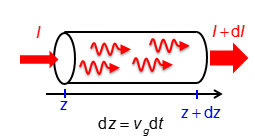
\includegraphics[scale=0.45]{ch3/image15}
	\captionof{figure}{ }
	\end{wrapfigure}
Attardons-nous quelque peu sur le $^{11}$Li. Considérons les rayons expérimentaux pour différents types de
Li et remarquons directement que le $^{10}$Li n'existe pas, celui-ci se désintègre directement. Entre 
$^9$Li et $^{11}$Li, l'écart est très important. Cette grand différence vient du fait que $^{11}$Li est à la
limite de la stabilité : l'énergie de liaison est toute petite et le rayon est donc grand. L'énergie de 
séparation de deux neutrons est également très petite, car les niveaux sont très proches. Il est possible de
comprendre ça en suivant un raisonnement très qualitatif en supposant qu'il n'y a qu'un seul neutron à 
l'extérieur? Il existe un potentiel $V(r)$ entre ces deux particules. Selon l'équation de \textsc{Schrödinger}
\begin{equation}
-\frac{\hbar^2}{2\mu}\psi'' + V(r)\psi = E\psi
\end{equation}
où $E=-\delta_m$, l'énergie de liaison. On ne connaît pas $V$, mais il est nul à grande distance. L'énergie étant
négative, la solution sera exponentielle. En supprimant l'exponentielle divergente
\begin{equation}
\psi \Rightarrow \exp(-kr)
\end{equation}
Faisons maintenant une grossière approche en supposant que ceci n'est pas valable à grande distance mais partout
et calculons-en le rayon carré moyen 
\begin{equation}
\langle r^2\rangle = \dfrac{\int |\psi|^2r^2 dr}{\int |\psi|^2 dr}
\end{equation}
En utilisant notre $\psi$ et par changement de variable, on voit que 
\begin{equation}
\langle r^2\rangle \propto 1/k^2
\end{equation}
Cette simple formule nous dit que quand l'énergie de liaison diminue, le rayon carré moyen (soit la taille du 
noyau) augmente. Ici le raisonnement tenu est très simple, mais qualitativement tout à fait valable.

\newpage
\section{Moments multipolaires}
Ces moments sont intimement liés à la déformation du noyau et sont utilisés pour tester les modèles 
nucléaires\footnote{Pas de notes sur cette dernière section, la précédente ok.}

\subsection{Moment quadrupolaire électrique}
Par définition ([e.fm$^2$])
\begin{equation}
Q = \sqrt{\dfrac{16\pi}{5}}e\bra{\Psi^{JJ\pi}}\sum_{i=1}^Z r_i^2Y_2^0(\Omega_i)\ket{\Psi^{JJ\pi}}
\end{equation}
Si $J<1$, alors par le théorème de \textsc{Wigner-Eckart} pour un OTI de rang 2, on en déduit que $Q=0$. Pour 
l'interprétation, il faut savoir que
\begin{equation}
r^2P_2(\cos\theta) = \frac{1}{2}(2z^2-x^2-y^2)
\end{equation}
Trois cas sont donc possibles
\begin{description}
\item[Q>0] Noyau allongé (\textit{prolate})
\item[Q<0] Noyau aplati
\item[Q=0] Noyau sphérique
\end{description}\ 

On peut ré-écrire l'élément de matrice dans le formalisme de l'isospin
\begin{equation}
\bra{\Psi^{JJ\pi}}\sum_{i=1}^Z r_i^2Y_2^0(\Omega_i)\ket{\Psi^{JJ\pi}} =
\bra{\Psi^{JJ\pi}}\sum_{i=1}^A \left(\frac{1}{2}-t_{iz}\right) r_i^2Y_2^0(\Omega_i)\ket{\Psi^{JJ\pi}}
\end{equation}
Par les propriétés du moment quadrupolaire, il est possible d'énoncer une définition alternative
\begin{equation}
\bra{\Psi^{JJ\pi}}\sum_{i=1}^Z r_i^2Y_2^0(\Omega_i)\ket{\Psi^{JJ\pi}} = \sqrt{\dfrac{4\pi}{5}}\int
\rho_{c,2}(r)r^2dr
\end{equation}
Le moment quadrupolaire est donné par le terme $\lambda=2$ de la densité de charge.

\subsection{Moment dipolaire magnétique}
Par définition
\begin{equation}
\mu = \sqrt{\dfrac{4\pi}{3}}\bra{\Psi^{JJ\pi}}M_0\ket{\Psi^{JJ\pi}}
\end{equation}
où $\vec{M} = \mu_N\sum_i(g_i\vec{l_i}+g_{si}\vec{s_i})$ avec $\mu_N=\frac{e\hbar}{m_Nc}$ le 
magnéton de \textsc{Bohr}, $g_s(n)=-3.82, g_s(p)=5.58$ les rapports gyromagnétiques et 
$g_l(i) = \frac{1}{2}-t_{iz}=0$ pour le neutron et 1 pour le proton. Si $J=0$ alors $\mu=0$ 
($\vec{M}$ est alors un opérateur de rang 1). Les moments quadrupolaire électrique et dipolaire 
magnétique sont utilisés pour tester les modèles nucléaires
\chapter{Interaction des photons avec la matière}
\section{Introduction}
\subsection{Considérations de bases et interactions des $\gamma$ avec la matière}
Les photons sont classifiés en fonction de leur origine
\begin{itemize}
\item[$\bullet$] Les $\gamma$ sont émis lors de transitions \textbf{nucléaires} $E_\gamma = 
E_i-E_f$ si on néglige l'énergie de recul du noyau. En général, $E_\gamma > 100$ keV.
\item[$\bullet$] Le Bremsstrahlung (rayons X de spectre continu, une particule peut perdre toute
son énergie en une fois) résulte de l'accélération d'une particule chargée.
\item[$\bullet$] Les rayons $X$ caractéristiques sont émis lors de transitions électroniques entre les couches atomiques $K, L, M, \dots$. En général, $E_X < 100$ keV.
\end{itemize}\ \\

	\begin{wrapfigure}[6]{r}{6.7cm}
	\vspace{-5mm}
	\includegraphics[scale=0.5]{ch4/image1}
	\captionof{table}{ }
	\end{wrapfigure}
La quantité de mouvement d'un photon vaut $\vec p = \hbar\vec{k}$ où $p = E_\gamma/c$ et $k$ est le
nombre d'onde. Ils interagissent avec la matière via des processus isolés, sans interactions entres-eux. 
Les photons sont des rayonnements \textbf{indirectement ionisants} : ils produisent des particules 
chargées qui, elles, vont ioniser la matière.\\

Pour des énergies entre le keV et le GeV, \textsc{Fano} a classifier 4 types d'interaction et 
3 conséquences de celle-ci, soit 12 processus théoriques possibles\footnote{Certains sont très 
rares, et d'autres n'ont jamais été observés.}. Sur ceux-ci, seuls trois effets dominent
\begin{enumerate}
\item \textit{L'effet Compton} (1B) : Le photon est diffusé par un électron libre ou faiblement lié.
La somme de l'énergie du photon et de l'énergie cinétique de l'électron est alors égale à l'énergie 
du photon incident
\item \textit{L'ffet photoélectrique} (1C) : Le photon est absorbé par un système électronique (atome). 
Il cède alors toute son énergie et un électron atomique\footnote{C'est-à-dire?} est éjecté hors de
l'atome avec une énergie cinétique égale à l'énergie du photon moins l'énergie de liaison de l'électron dans l'atome.

\item \textit{La création de paire} (3C) : Le photon disparait dans le champ électrique d'un noyau 
ou d'un électron et une paire électron-positron apparaît.
\end{enumerate}

Deux autres processus peuvent aussi jouer un rôle
\begin{enumerate}
\item \textit{Diffusion de Rayleigh} (1A) : Le photon est dévié sans perte d'énergie par un système
électronique (atome)
\item \textit{Photodésintégration du noyau}(2C): Le photon est absorbé par le noyau et une particule est émise ($\gamma, \alpha, p, n,\dots)$.
\end{enumerate}
On ne parlera pas du dernier point car l'énergie concernée est bien supérieure à celle utilisée en
métrologie nucléaire.


\subsection{Remarque importante}
Un photon \textbf{ne} peut \textbf{pas} être absorbé par un électron libre et lui céder toute son 
énergie. Par conservation de l'énergie et de l'impulsion avec $h\nu_0$ l'énergie du photo et $m,E$ et 
$p$, la masse, l'énergie totale et l'impulsion de l'électron on peut écrire
\begin{equation}
h\nu_0+mc^2=E,\qquad\qquad \dfrac{h\nu_0}{c}=p
\end{equation}
Ce qui implique que $E=pc+mc^2$. Or, par définition $E^2=p^2c^2+m^2c^4$. L'absorption serait possible
que pour $p=h\nu_0=0$ ce qui est à rejeter. 



\section{Effet Compton}%sl10
	\begin{wrapfigure}[6]{r}{4cm}
	\vspace{-10mm}
	\includegraphics[scale=0.4]{ch4/image2}
	\captionof{figure}{ }
	\end{wrapfigure}
L'effet \textsc{Compton} est un scattering par un électron libre dans une certaine plage énergétique
où les électrons sont considérés comme libre\footnote{Lorsque ce n'est plus le cas, l'effet 
photoélectrique domine}. Le photon incident est donc diffusé (au sens du scattering) et cède une 
partie de son énergie à un électron.\\

C'est en \textit{1906} que \textsc{Thomson} calcula classiquement la section efficace de diffusion
d'une onde électromagnétique par un électron libre. Un électron oscille en réponse à la force
exercée par le champ électrique de l'onde, à la même fréquence que celui-ci. Il en résulte un 
dipôle magnétique faisant que l'électron rayonne causant une diffusion continue\footnote{L'idée 
est bonne, mais nous verrons que ceci est faux.} de l'onde incidente.\\

Pour une onde non polarisée, la section efficace de diffusion \textsc{Thomson} s'écrit
\begin{equation}
\frac{d\sigma_0}{d\Omega}=\frac{r_e^2}{2}(1+\cos^2\theta)
\end{equation}
où $r_e = e^2/4\pi\epsilon_0mc^2$, le rayon classique de l'électron. 

	
\subsection{Démonstration de Thomson}
Soit une onde électromagnétique de fréquence $\nu$ interagissant avec un électron libre de 
masse $m$ et charge $-e$
\begin{equation}
\overrightarrow{E}=E_0\exp{(i\overrightarrow{k}\overrightarrow{r}-i\nu t)}\overrightarrow{1_E}
\end{equation}
où $\vec{1_E}$ est la direction de polarisation. L'électron subit une force $\vec{F}$ à cause
de ce champ, son équation du mouvement s'écrit
\begin{equation}
m\frac{d^2\overrightarrow{r}}{dt^2}=-e\overrightarrow{E}
\end{equation}
Dans l'approximation dipolaire la puissance émise par unité d'angle solide s'écrit (formule 
de \textsc{Larmor} différentielle - voir cours d'électromagnétisme) 
\begin{equation}
\frac{dP}{d\Omega}=\frac{e^2}{16\pi^2\epsilon_0c^3}\langle a^2 \rangle \sin^2\Theta
\end{equation}
où $\Theta$ est l'angle entre la direction de polarisation et l'observateur. On peut directement
obtenir la moyenne de l'accélération au carré avec l'équation de mouvement
\begin{equation}
\langle a^2 \rangle=\frac{e^2}{2m^2}|E_0|^2
\end{equation}
En remplaçant dans la précédente équation, on trouve la puissance différentielle
\begin{equation}
\frac{dP}{d\Omega}=r_e^2 \frac{\epsilon_0c|E_0|^2}{2}\sin^2\Theta
\end{equation}
En considérant le module du vecteur de Poynting $I=\epsilon_0c\frac{|E_0|^2}{2}$ et en substituant
son expression, on trouve la section efficace différentielle
\begin{equation}
\frac{d\sigma_0}{d\Omega}=\frac{dP/d\Omega}{I}=r_e^2\sin^2\Theta
\end{equation}
Pour une onde incidente non-polarisée, il faut prendre la moyenne de $\Theta$
\begin{equation}
\overline{\sin^2\Theta}=\frac{1}{2}(1+\cos^2\theta)
\end{equation}
où $\theta$ est l'angle de scattering. En remplaçant on trouve l'équation de \textsc{Thomson}, 
purement classique
\begin{equation}
\frac{d\sigma_0}{d\Omega}=\frac{r_e^2}{2}(1+\cos^2\theta)
\end{equation}
L'intégration sur tout les angles possible donne la section efficace totale de diffusion
\textsc{Thomson}
\begin{equation}
\sigma_0=\frac{8\pi}{3}r_e^2=0.665\times 10^{-28} \mbox{~m}^2 \approx \frac{2}{3} \mbox{~~barn/\'electron}
\end{equation}
Le problème est la diffusion continue de l'onde incidente, comme \textsc{Compton} va faire remarquer.

\subsection{Expérience de Compton}%sl16
En \textit{1922}, \textsc{Compton} mesure les longueurs d'onde des rayonnements incidents et diffusés
et montre que le spectre n'est pas continu mais suit
\begin{equation}
\lambda_1-\lambda_0=\frac{h}{mc}(1-\cos\theta)
\end{equation}
où $\lambda_0, \lambda_1$ sont les longueurs d'ondes des photons incidents et diffusés et $\lambda_C$, 
la longueur d'onde de \textsc{Compton}. La diffusion par un électron ne dépend pas du nombre 
atomique du diffuseur, ni de la longueur de l'onde incidente :  l'énergie et l'impulsion perdue par
le photon se retrouvent dans un seul électron.

\subsubsection{Démonstration de l'expression de Compton}
Plaçons-nous dans le référentiel du laboratoire et écrivons les quadrivecteurs associés
\begin{eqnarray}
\mbox{photon avant} &\rightarrow& \left(\frac{h\nu_0}{c},\frac{h\nu_0}{c}\overrightarrow{n_0}\right)\\
\mbox{photon apr\`es} &\rightarrow& \left(\frac{h\nu_1}{c},\frac{h\nu_1}{c}\overrightarrow{n_1}\right)\\
\mbox{\'electron avant} &\rightarrow& \left(\frac{mc^2}{c},0\right)\\
\mbox{\'electron apr\`es} &\rightarrow& \left(\frac{E}{c},\overrightarrow{p}\right)
\end{eqnarray}
Par conservation de l'énergie et de l'impulsion
\begin{eqnarray}
h\nu_0+mc^2=h\nu_1+E\\
h\nu_0\overrightarrow{n_0}=h\nu_1\overrightarrow{n_1}+\overrightarrow{p}c
\end{eqnarray}
Avec $E^2=p^2c^2+m^2c^4$, en isolant $p$ :
\begin{equation}
(h(\nu_0-\nu_1)+mc^2)^2=h^2(\nu_0\overrightarrow{n_0}-\nu_1\overrightarrow{n_1})^2+m^2c^4
\end{equation}
Sachant que $\overrightarrow{n_0}\overrightarrow{n_1}=\cos{\theta}$, on trouve
\begin{equation}
h\nu_0\nu_1(1-\cos\theta)=mc^2(\nu_0-\nu_1)\Rightarrow \frac{hc^2}{\lambda_0\lambda_1}(1-\cos\theta)=mc^3\left(\frac{1}{\lambda_0}-\frac{1}{\lambda_1}\right)
\end{equation}
Et donc
\begin{equation}
\lambda_1-\lambda_0=\frac{h}{mc}(1-\cos\theta)
\end{equation}

\subsection{Relations entre énergies et angles}%sl19
Soit $E_0$ et $E_1$ les énergies du photon indicent et diffusé, $T=E_0-E_1$ l'énergie cinétique 
cédée à l'électron, $\theta$ l'angle de diffusion du photo, $\phi$ l'angle entre la trajectoire de
l'électron et la direction initiale du photon et $\alpha=E_0/mc^2$. On peut écrire
\begin{equation}
T=E_0\frac{2\alpha \cos^2\phi}{(1+\alpha)^2-\alpha^2\cos^2\phi}=E_0\frac{\alpha(1-\cos\theta)}{1+\alpha(1-\cos\theta)}
\end{equation}\ 

	\begin{wrapfigure}[14]{l}{8.5cm}
	\vspace{5mm}
	\includegraphics[scale=0.45]{ch4/image3}
	\captionof{figure}{ }
	\end{wrapfigure}
	\ 
	
\begin{equation}
E_1=E_0\frac{1}{1+\alpha (1-\cos\theta)},\quad 
\cot\phi=(1+\alpha)\tan\frac{\theta}{2}
\end{equation}

Ces formules représentées graphiquement donnent déjà un bon nombre d'informations. Comme $0<\theta<
\pi$, on sait que $(E_1)_{min} = E_0/(1+2\alpha)$ et $(E_1)_{max} : E_0$. Lorsque l'angle augmente, 
$E_1$ a tendance à diminuer. L'effet de l'angle se marque assez peu à faible énergie mais devient
significatif à haute énergie. La ligne bleue correspond à une rétro-diffusion, ce point sera
abordé plus tard.

\newpage
\textsc{Remarques}
\begin{itemize}
\item[$\bullet$] Le déplacement en longueur d'onde ne dépend pas de l'énergie du photon incident 
(uniquement de l'angle de diffusion)
\item[$\bullet$] Le déplacement en énergie dépend fortement de l'énergie du photon incident et 
augmente fortement avec l'énergie
\item[$\bullet$] Pour $E_0$ petit, le photon perd peu d'énergie $\forall\theta$
\item[$\bullet$] Lorsque $E_0$ augmente, la variation de l'énergie du photon diffusé avec l'angle
 devient de plus en plus rapide
\item[$\bullet$] A $90^\circ$, $E_1 < 511$ keV (toujours, =$mc^2$)
\item[$\bullet$] A $180^\circ$, $E_1 < 255$ keV (toujours, =$mc^2/2$). Il s'agit de la
rétro-diffusion du photon et explique le pic de rétro-diffusion dans les spectres $\gamma$.
\end{itemize}\ 

	\begin{wrapfigure}[8]{r}{6cm}
	\vspace{-7mm}
	\includegraphics[scale=0.5]{ch4/image4}
	\captionof{figure}{ }
	\end{wrapfigure}
	
Regardons $\phi$. On observe que $0<\phi<\pi/2$ impliquant $T_{min}=0$ et \\

\retenir{\begin{equation}
T_{max} = \dfrac{E_0}{1+(1/2\alpha)}
\end{equation}
A retenir car pratique pour tracer des spectres!}\ \\

Ci-contre, la représentation de la variation de l'énergie maximale de l'électron en fonction 
de l'énergie du photon indicent. On remarque que la déviation du photon se fait dans le sens
de la trajectoire pour les grandes énergies (et donc faible angle).\\



\subsection{Section efficace différentielle angulaire, énergétique et totale}
\subsubsection{Section efficace différentielle angulaire} %sl25
Il s'agit de la première chose qui a été calculé par \textsc{Klein-Nishina} (valable pour 
des électrons libres et au repos) via la théorie quantique relativise et l'équation de
\textsc{Dirac}.

\begin{center}
	\includegraphics[scale=0.6]{ch4/image5}
	\captionof{figure}{Plus on monte en énergie, plusla direction privilégiée est dnas le sens de la trajectoire (droite).}
\end{center}

\newpage
La section efficace différentielle de diffusion d'un photon (non polarisé) par un électron dans
l'angle solide d$\Omega$ autour de la direction formant un angle $\theta$ avec la direction initiale
du photon est donnée par 
\begin{equation}
\frac{d\sigma}{d\Omega}=\frac{r_e^2}{2}\left(\frac{\nu'}{\nu_0}\right)\left(\frac{\nu_0}{\nu'}+\frac{\nu'}{\nu_0}-\sin^2\theta\right)
\end{equation}
où $r_e$ est le rayon classique de l'électron. Notons la non-dépendance en $Z$. Pour de très faibles
énergie ($\alpha\ll 1$), $E_1\approx E_0$ impliquant que d$\sigma \approx$ d$\sigma_0$ : on 
retrouve la section efficace de \textsc{Thomson} ! Celle-ci n'était donc pas si mauvaise car on la
retrouve à faible énergie.

\subsubsection{Section efficace différentielle énergétique}%sl28
A partir de la section efficace différentielle en angle, on peut trouver les sections différentielles
en énergie. Rien de compliqué, mais rien de drôle non plus
\begin{equation}
\frac{d\sigma}{dE_1}=\frac{\pi r_e^2}{\alpha^2m_ec^2}\left\{2+\left(\frac{E_0-E_1}{E_1}\right)^2\left[\frac{1}{\alpha^2}+\frac{E_1}{E_0}-\frac{2}{\alpha}\left(\frac{E_1}{E_0-E_1}\right) \right]\right\}
\end{equation}
Par changement de variable (à faire un samedi soir)
\begin{equation}
\frac{d\sigma}{dT}=\frac{\pi r_e^2}{\alpha^2m_ec^2}\left\{2+\left(\frac{T}{E_0-T}\right)^2\left[\frac{1}{\alpha^2}+\frac{E_0-T}{E_0}-\frac{2}{\alpha}\left(\frac{E_0-T}{T}\right) \right]\right\}
\end{equation}
La représentation graphique (slide 29) montre que cette section efficace est assez équiprobable pour
de faibles énergies. Plus l'énergie augmente, plus il y a un pic prononcé lorsque l'on arrive à
la valeur du seuil \textsc{Compton}.

\subsubsection{Section efficace différentielle totale}%sl30
Après intégration de la section efficace de \textsc{Klein-Nishina} sur les angles
\begin{equation}
\sigma=2\pi r_e^2\left\{\frac{1+\alpha}{\alpha^2}\left[\frac{2(1+\alpha)}{1+2\alpha}-\frac{\ln{(1+2\alpha)}}{\alpha}\right]+\frac{\ln{(1+2\alpha)}}{2\alpha}-\frac{1+3\alpha}{(1+2\alpha)^2}\right\}
\end{equation}
Pour $\alpha\ll 1 \to \sigma \approx \sigma_0$, la section efficace de \textsc{Thomson}. Pour
$\alpha\gg 1, \sigma  \to (\ln\alpha)/\alpha$, la section efficace de \textsc{Compton} décroit
lorsque l'énergie du photon augmente. Si on regarde les précédents graphique, la distribution
est piquée en $\theta=0$ ce qui répond au cas où il n'y a ni diffusion, ni transfert d'énergie et
donc pas d'effet. Notons que la section efficace \textbf{atomique} est proportionnelle à $Z$.\\

La section efficace $\sigma$ représente la probabilité de collision, soit le cas où une partie de
l'énergie est diffusée et l'autre est cédée à l'électron (absorbée). La collision reprend donc 
la diffusion, mais également l'absorption. Pour caractériser cet aspect, on défini une section
efficace de diffusion $\sigma_s$ et d'absorption $\sigma_a$ tel que $\sigma = \sigma_s+\sigma_a$.



\subsection{Diffusion cohérente et incohérente}%sl32

Pour de très faibles énergies $E_0$, d'électron est de moins en moins libre/au repos et les anciennes 
hypothèses tombent à l'eau, il va falloir prendre en considération le système électronique tout
entier et non plus . Deux cas sont possibles
\begin{enumerate}
\item L'atome reste dans son état intial et le photo est juste dévie : diffusion de 
\textsc{Rayleigh} (\textbf{cohérente})
\item L'atome change d'état : le photon perd de l'énergie, la diffusion est \textbf{incohérente}
\end{enumerate}
Pour de grandes énergies, on nomme la diffusion incohérente la diffusion \textsc{Compton}.\\

	\begin{wrapfigure}[15]{r}{8cm}
	\vspace{-5mm}
	\includegraphics[scale=0.5]{ch4/image6}
	\captionof{figure}{ }
	\end{wrapfigure}
	
En guise de première approximation pour la diffusion cohérente, on peut voir le système électronique
comme un système de charge $Ze$ et de masse $Zm$. La section efficace de Rayleigh vaut alors
\begin{equation}
_a\sigma_{coh}=Z^2\sigma_0
\end{equation}
En réalité la structure du nuage électronique implique une diminution de la diffusion et l'on utilise
\begin{equation}
_a\sigma_{coh}=F^2\sigma_0
\end{equation}
Pour la diffusion incohérente, on modifie la section efficace de \textsc{Klein-Nishina} en 
introduisant la fonction de diffusion incohérente $S$ tenant compte du fait qu'un 
photon peut éjecter un électron
\begin{equation}
_a\sigma_{incoh}=Z\sigma S
\end{equation}


\section{Effet photoélectrique}%sl38
	\begin{wrapfigure}[7]{l}{5cm}
	\vspace{-5mm}
	\includegraphics[scale=0.5]{ch4/image7}
	\captionof{figure}{ }
	\end{wrapfigure}
L'\textbf{effet photoélectrique} est un processus au cours duquel un photon incident interagit avec 
un atome et éjecte un électron (processus expliqué correctement par \textsc{Einstein} en 
\textit{1905}), souvent appelé \textit{photoélectron}. Ce processus de capture d'un photon par un
atome dont un électron est excité dans un état continu est le processus inverse de l'émission spontanée d'un photon par un atome excité


\subsection{Conservation de l'énergie et énergie de liaison} %sl39
	\begin{wrapfigure}[15]{r}{7cm}
	\vspace{-5mm}
	\includegraphics[scale=0.5]{ch4/image8}
	\captionof{figure}{Pour $Z > 30$, les énergies de liaison obéissent approximativement à 
	$B_i = a_i(Z-c_i)^2$ (avec $a_i$ et $c_i$, des constantes pour chaque couche)}
	\end{wrapfigure}
Soit l'absorption totale d'un photon d'énergie $h\nu_0$ causant l'émission d'un électron avec une
énergie cinétique $T$ hors d'une couché atomique caractérisée par une énergie de liaison $B_i$. En
négligeant l'énergie du recul du noyau
\begin{equation}
h\nu_0=T+B_i
\end{equation}
Par conservation, il faut que $h\nu_0>B_i$. Ainsi lorsque $h\nu_0$ augmente, la probabilité de l'effet
photoélectrique diminue car le comportement de l'électron se rapproche plus de celui d'un électron
libre (et celui-ci \textbf{ne} peut \textbf{pas} se faire totalement absorbé). A priori on regarde 
plus les couches externes (couche $K\to B_K$), ceux-ci possédant une énergie de liaison plus faible.

\newpage
\subsection{Section efficace}%sl41
On peut décomposer la section efficace par atome $_a\tau$ en une somme de sections efficaces 
partielles $_a\tau_i$ correspondant à l'éjection d'une électron hors d'une couche $i$
\begin{equation}
_a\tau=\sum_i {}_a\tau_i
\end{equation}	
Le calcul de $_a\tau_K$ a été fait pour un atome hydrogénoïde dans 	l'approximation de \textsc{Born}
en utilisant une onde plane comme fonction d'onde de l'électron éjecté : pas le choix, la fonction
d'onde de l'électron est trop compliquée. Restreignons la zone de travail en énergie en faisant
l'approximation non relativiste et que l'interaction noyau/électron est négligeable : $\B_k\ll 
\hbar\nu_0\ll mc^2$. On trouve (cadeau)
\begin{equation}
_a\tau_K=\frac{8\pi}{3}\left(\frac{a_0}{Z}\right)^232\alpha\left(\frac{B_K}{h\nu_0}\right)^{7/2}
\end{equation}
Lorsque l'approximation de \textsc{Born} n'est plus valable, il faut introduire un facteur correctif
\begin{equation}
f(\xi)=2\pi\left(\frac{B_K}{h\nu_0}\right)^{1/2}\frac{e^{-4\xi \text{arccot}{\xi}}}{1-e^{-2\pi \xi}}\mbox{~~avec~~}\xi=\left(\frac{B_K}{h\nu_0-B_K}\right)^{1/2}
\end{equation}
En pratique pas grand monde s'intéresse à ceci, même ceux qui travaillent dans le domaine 
utilisent les valeurs de tables et ne font pas trop attention à la forme. Ce qui est intéressant
c'est que $a_0/Z$ est grossièrement la dimension de l'atome et que l'énergie varie en 
$h\nu_0^{7/2}$.\\


	\begin{wrapfigure}[10]{r}{7cm}
	\vspace{-5mm}
	\includegraphics[scale=0.5]{ch4/image9}
	\captionof{figure}{Variation de $_a\tau$ avec $h\nu_0$}
	\end{wrapfigure}
	
Les autres section efficaces partielles suivent le même comportement, on les note sous la forme\\

\retenir{
\begin{equation}
_a\tau=C\frac{Z^n}{(h\nu_0)^k}
\end{equation}
où $4<n<4.6$ et $1<k<3$.}\ \\

Cette formule est intéressante à retenir car elle montre une forte dépendance en énergie mais 
également une dépendance en $Z$. Ces constantes sont difficile à trouver, on sait que l'énergie 
doit être en proche (en puissance) de $-7/2$ mais on en sait pas plus. 


\subsection{Distribution angulaire des photoélectrons}
On se rappelle que - dans l'approximation de \textsc{Born} - la section efficace différentielle
est proportionnelle à
\begin{equation}
f(\theta)=\frac{\sin^2\theta}{(1-\beta\cos\theta)^4}
\end{equation}
La section efficace s'annule dans la direction du photon indicent $\theta=0$ ce qui est une 
conséquence de la nature transverse des ondes électromagnétiques. L'électron tend donc à être
éjecté dans la direction du champ $\vec{E}$ de cette onde\footnote{Notons que, physiquement, 
$\theta=0$ est impossible.}. Dans le cas relativiste
\begin{equation}
f(\theta)=\frac{\sin^2\theta}{(1-\beta\cos\theta)^4}+\frac{3(1-\sqrt{1-\beta^2})-2\beta^2}{2(1-\beta^2)^{3/2}}\times\frac{\sin^2\theta}{(1-\beta\cos\theta)^3}
\end{equation}
\newpage
	\begin{wrapfigure}[7]{r}{4.5cm}
	\vspace{-3mm}
	\includegraphics[scale=0.5]{ch4/image10}
	\captionof{figure}{ }
	\end{wrapfigure}

Que ce soit relativiste ou non, lorsque l'énergie des photons augmente de plus en plus d'électrons
sont éjectés vers l'avant. \\

On nomme \textbf{angle de bipartition} $\theta_b$ l'angle pour lequel la moitié des photoélectrons
sont émis vers l'avant dans un cône de demi-angle inférieur à $\theta_b$.



\subsection{Phénomène consécutif à l'effet photoélectrique}%sl53
	\begin{wrapfigure}[9]{l}{9.8cm}
	\vspace{-5mm}
	\includegraphics[scale=0.5]{ch4/image11}
	\captionof{figure}{ }
	\end{wrapfigure}
L'émission d'un électron à cause d'un photoélectrique crée un trou dans une couche interne. Après
réarrangement électronique, il y a émission d'un rayon $X$ (fluorescence) \textit{ou} d'un électron
\textsc{Auger}. On défini alors un \textbf{rendement de fluorescence} $\omega_i$ qui est la 
probabilité d'émission d'un photon après une transition vers la couche $i$. Ce rendement est faible
pour les matériaux à petit $Z$.


\section{Création de paire}%sl 55
	\begin{wrapfigure}[5]{r}{5.6cm}
	\vspace{-5mm}
	\includegraphics[scale=0.5]{ch4/image12}
	\captionof{figure}{ }
	\end{wrapfigure}
La création de paire se produit dans le champ électrique du noyau ou d'un électron atomique (plus 
rarement, on parlera de création de triplet où une partie de l'énergie est transférée à l'électron
initial)), le photon disparaît alors et il se forme une paire
électron-positron. 

\subsection{Lois de conservation}%sl56
Afin de déterminer l'énergie minimale du photon incident pour avoir création de paire, écrivons 
les équations de conservation. Avant l'interaction, on travaille dans le repère de la particule
cible de masse $M$, au repos
\begin{eqnarray}
\mbox{photon avant} &\rightarrow& \left(\frac{h\nu_0}{c},\frac{h\nu_0}{c}\right)\\
\mbox{particule cible avant} &\rightarrow& \left(\frac{Mc^2}{c},0\right)
\end{eqnarray}
Après l'interaction, on se place dans le référentiel du centre de masse
\begin{eqnarray}
\mbox{\'electron apr\`es} &\rightarrow& \left(\frac{mc^2+T_e}{c},\overrightarrow{p_e}\right)\\
\mbox{positron apr\`es} &\rightarrow& \left(\frac{mc^2+T_p}{c},\overrightarrow{p_p}\right)\\
\mbox{particule cible apr\`es} &\rightarrow& \left(\frac{Mc^2+T_C}{c},\overrightarrow{p_C}\right)
\end{eqnarray}
Après le choc, en travaillant dans le référentiel du centre de masse\footnote{Égalité nulle car
init. au repos?}
\begin{equation}
\overrightarrow{p_e}+\overrightarrow{p_p}+\overrightarrow{p_C}=0
\end{equation}
En notant $T_{tot} = T_e+T_p+T_C$ et par conservation de l'invariant $P^2=(E/c)^2+p^2$
\begin{eqnarray}
\mbox{avant} &\rightarrow& P^2=\left(\frac{h\nu_0}{c}+\frac{Mc^2}{c}\right)^2-\left(\frac{h\nu_0}{c}\right)^2\\
\mbox{apr\`es} &\rightarrow& P^2=\left(\frac{2mc^2+Mc^2+T_{tot}}{c}\right)^2
\end{eqnarray}
On trouve l'énergie minimale $h\nu_{m,min}$ en égalant les deux expression pour $T_{tot}=0$
\begin{equation}
h\nu_{0,min}=2mc^2\left(1+\frac{m}{M}\right)
\end{equation}
où $m$ est la masse de l'électron et $M$ celle de la particule cible
En conclusion
\begin{itemize}
\item[$\bullet$] \textit{Dans le champ d'un noyau} : $M\gg m \to h\nu_{0,min} = 2mc^2$
\item[$\bullet$] \textit{Dans le champ d'un électron} : $M= m \to h\nu_{0,min} = 4mc^2$
\end{itemize}
Ce phénomène est aussi possible entre $2mc^2$ et $4mc^2$ car l'atome peut prendre avec lui
une fraction de la quantité de mouvement initiale, mais c'est très rare.

\subsection{Section efficace dans le champ d'un noyau}%sl59
Le calcul de la section efficace \textsc{Compton} était déjà sympathique, ici c'est pire. On se
contentera de donner les résultats important sans faire de calculs détaillés. La raison est que 
c'est compliqué notamment à cause du nuage électronique qui a des effets d'écrantage des électrons
atomiques. \\

Lorsqu'on regarde les spectres de l'électron et du positron, ils sont décalés. On peut négliger cette
différence et considérer la section efficace différentielle pour la création d'un électron à énergie
cinétique $T_-$ est identique à celle de création d'un positron à énergie cinétique $T_+=h\nu_0-2mc-
T_-$. Cette section efficace différentielle est symétrique par rapport à 
\begin{equation}
\langle T \rangle = \frac{h\nu_{0}-2mc^2}{2}
\end{equation}
En s'amusant un peu
\begin{equation}
\frac{d{}_a\kappa}{dT_+}=\frac{\sigma_pZ^2P(T_+,h\nu_0,Z)}{h\nu_0-2mc^2}{\mbox{~~~~pour~~~~}}h\nu_0>2m_ec^2
\end{equation}
où encore
\begin{equation}
\frac{d{}_a\kappa}{dx}=\sigma_pZ^2P(x,h\nu_0,Z)
\end{equation}
avec $x = T_+/(h\nu_0-2m_ec^2)$.\\

	\begin{wrapfigure}[6]{r}{3cm}
	\vspace{-5mm}
	\includegraphics[scale=0.24]{ch4/image13}
	\captionof{figure}{ }
	\end{wrapfigure}
Intéressons-nous quelque peu à la fonction $P(x,h\nu_0,Z)$ représentée ci-contre. Il s'agit d'une
fonction symétrique qui ne dépend que peu de $Z$ : la section efficace est $\propto Z^2$. Cette 
fonction est lentement variable en l'énergie $h\nu_0$ du photon et est approximativement constante
pour $0.2<x<0.8$.

\newpage
\subsection{Section efficace totale}%sl63	
Si on veut la section efficace totale, il faut intégrer sur l'énergie $T_+$
\begin{eqnarray}
{}_a\kappa&=&\int_{T_+}d{}_a\kappa=\sigma_pZ^2\int_0^{h\nu_0-2mc^2}\frac{PdT_+}{h\nu_0-2mc^2}\\
&=&\sigma_pZ^2\int_0^{1}Pd\left(\frac{T_+}{h\nu_0-2mc^2}\right)\\
&=&\sigma_pZ^2\langle P\rangle
\end{eqnarray}
où $\langle P\rangle$ est la valeur moyenne de $P$. Celle-ci dépend très peu de $Z$ est est 
une fonction lentement croissante de $h\nu_0$ avant de devenir constante à grande énergie 
(>100 MeV) à cause de l'écrantage.




\subsection{Section efficace dans la champ d'un électron}
Le calcul est très compliqué mais on peut montrer que
\begin{equation}
{}_a\kappa_{triplet}=\sigma_pZ\langle P\rangle_{triplet}{\mbox{~~~~pour~~~~}}h\nu_0>4m_ec^2
\end{equation}
et donc que
\begin{equation}
\frac{{}_a\kappa_{triplet}}{{}_a\kappa}\simeq \frac{1}{CZ}
\end{equation}
où $C$ est un paramètre seulement fonction de $h\nu_0$. Ce qui est important c'est que 
la création de paire dans le champ des électrons ne contribue que peu à la section efficace 
totale de création de paire sauf pour les matériaux à $Z$ petit 

\subsection{Direction d'émission de la paire électron-positron}%sl67
	\begin{wrapfigure}[6]{l}{6cm}
	\vspace{-5mm}
	\includegraphics[scale=0.24]{ch4/image14}
	\captionof{figure}{ }
	\end{wrapfigure}
	
Pour des photons d'énergie $h\nu_0$ largement supérieur à l'énergie de seuil, les électrons et 
positrons sont fortement émis vers l'avant. Leur angle d'émission moyen relatif à la direction
d'origine du photon vont grossièrement (rad.)
\begin{equation}
\langle \theta \rangle \simeq \frac{mc^2}{\langle T \rangle}
\end{equation}






\subsection{Phénomène consécutif à la création de paire et photodésintégration du noyau} 
\subsubsection{Phénomène consécutif à la création de paire}
Très brièvement, le positron s'annihile avec un électron (au repos) lorsqu'il traverse la matière mais 
avant ça il ralenti car les collisions sont nettement plus probables que l'annihilation. Cette
dernière se produit le plus souvent lorsque le positron est \textit{quasi au repos} et deux 
photons de 511 keV sont produits à 108$^\circ$ l'un de l'autre.

\subsubsection{Photodésintégration du noyau}
Le photon est absorbé par un noyau et une particule est émise (un photon ou une particule légère (p,
n,$\alpha$, \dots) mais il faut une énergie entre 8 et 20 MeV(!).

\subsection{Comparaison des différents effets}
Commenter le graphique est une bonne question d'examen. Voir notes, slide 70 (beaucoup à dire, je 
n'ai pas le temps de le faire pour le moment).


\section{Coefficient d'atténuation}
Nous venons de voir trois processus d'interaction d'un photon dans la matière et leurs sections
efficaces
\begin{enumerate}
\item Effet photoélectrique : $_a\tau$
\item Effet \textsc{Compton} : $_a\sigma = Z\sigma$
\item Création de paire : $_a\kappa$
\end{enumerate}
où $_a$ signifie atomique. Les autres processus étant négligeable, la section efficace totale
n'est que la somme de ces trois effets
\begin{equation}
{}_a\mu={}_a\tau+{}_a\sigma+{}_a\kappa
\end{equation}
La probabilité qu'un photon ait une interaction dans une cible mince de densité $N$ et d'épaisseur
$dx$ vaut $_a\mu Ndx$. Pour un faisceau monocinétique de $I$ photons par unité de temps, le taux 
de collision vaut $I_a\mu Ndx$. La variation d$I$ d'intensité après avoir quitté la cible vaut 
alors $dI = -I_a\mu Ndx$. Pour une cible finie et un faisceau initial perpendiculaire à la cible
de $I_0$ particules, l'intensité après le passage dans la cible est
\begin{equation}
I=I_0\exp{(-_a\mu Nl)}
\end{equation}
où $\mu = _a\mu N$ est le \textbf{coefficient linéique d'atténuation} (m$^{-1}$) qui nous 
informe sur la \textit{fréquence des collisions}.

\subsection{Géométrie à faisceau étroit}
	\begin{wrapfigure}[9]{l}{7cm}
	\vspace{-5mm}
	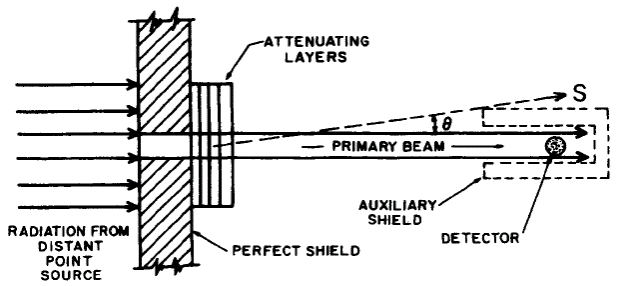
\includegraphics[scale=0.4]{ch4/image16}
	\captionof{figure}{ }
	\end{wrapfigure}
Pour vérifier cette loi, il faut utiliser une \textit{géométrie à faisceau étroit} empêchant les
qui empêche les particules primaires déviées et les secondaires d'attendre le détecteur (on 
ne veut pas qu'un électron arraché à la cible soit détectée). Pour se faire il faut une grande 
distance entre la source et l'atténuateur, de même entre l'atténuateur et le détecteur et le 
faisceau doit recouvrir tout le détecteur uniformément. De même, on utilise un blindage devant
l'atténuateur pour stopper les rayons incident exceptés ceux passant par l'ouverture et un 
blindage autour du détecteur pour stopper les rayons $X$ ou $\gamma$.

\subsection{Coefficient massique d'atténuation}%78
On définit le \textbf{coefficient massique d'atténuation} comme le rapport $\rho/\mu$ 
(m$^2$.kg$^{-1}$). Il s'agit du quotient de $dI/I$ par $\rho dI$ où $dI/I$ est la fraction de
particules indirectement ionisantes qui subissent des interactions le long de la distance d$l$ 
parcourue dans un matériau de masse volumique $\rho$. Il s'agit du coefficient \textbf{le plus
important}.\\

Il s'agit d'un coefficient global qui prend en compte les interactions des particules dans la 
matière sans préciser la nature de l'interaction. Ils sont directement proportionnel à la 
section efficace et ne dépendent \textbf{pas} de la nature de la cible !

\newpage
Si le matériau contient plusieurs espèces atomiques, on somme les probabilités d'interaction 
de chaque type d'atomes. Le coefficient massique d'atténuation total est alors donén par
\begin{equation}
\left(\frac{\mu}{\rho}\right)=\left(\frac{\mu}{\rho}\right)_1w_1+\left(\frac{\mu}{\rho}\right)_2w_2+
\dots
\end{equation}
où $w_i$ sont les fractions massiques des différentes espèces d'atomes.

\subsection{Coefficient de transfert massique d'énergie}%sl83
Le coefficient d'atténuation massique mesure le nombre moyen d'interaction entre un photon 
et la matière, il permet donc d'évaluer la fréquence des collisions. Souvent on s'intéresse
à l'énergie déposée "localement"\footnote{Ici quasi uniquement dues aux effets des électrons 
produits.}. On définit alors le \textbf{coefficient de transfert massique d'énergie} $\mu_{tr}/\rho$.
On le défini aussi comme\footnote{Voir slide 84 pour plus de détails, peu de notes}
\begin{equation}
\frac{\mu_{tr}}{\rho}=f_{ph}\frac{\tau}{\rho}+f_{C}\frac{\sigma}{\rho}+f_{pn}\frac{\kappa_n}{\rho}+f_{pe}\frac{\kappa_e}{\rho}
\end{equation}
avec $f_i$, les fractions d'énergie du photon transférées sous forme d'énergie cinétique à des
particules chargées pour chaque processus. Pour les trois processus étudiés
\begin{enumerate}
\item Effet photoélectrique
\begin{equation}
f_{ph}=1-\frac{E_X}{E}
\end{equation}
où $E_X$ est l'énergie moyenne des photons de fluorescence. Tout l'énergie est cédée à l'électron, 
sauf celle cédée au rayon $X$.
\item Effet \textsc{Compton}
\begin{equation}
f_{C}=1-\frac{\langle E_1 \rangle +E_X}{E}
\end{equation}
avec $\langle E_1\rangle$ l'énergie du photon diffusé. Il s'agit de (ce qui est émis)-(ce qui est
diffusé). Notons que le $E_X$ peut être négligé en pratique. 
\item Création de paire
\begin{equation}
f_{pn}=1-\frac{2mc^2}{E},\qquad\qquad\qquad f_{pe}=1-\frac{2mc^2+E_X}{E}
\end{equation}
(Tout)-(énergie servant à créer la paire). Ici on ne peut pas négliger le rayon $X$ car ça dépend
ou s'est formée la paire (alors que \textsc{Compton} concernait les électrons moins liés).
\end{enumerate}\ \\

Une fraction de l'énergie cinétique emportée par les particules chargées mises en mouvement lors des
interactions des particules primaires avec le matériau peut ne pas être absorbée localement. Une
partie de leur énergie peut alors être émise sous forme de rayonnement de freinage (surtout pour des 
électrons secondaires d'énergie élevée). Il faut alors corriger le précédent coefficient pour tenir
compte de ces rayonnements
\begin{equation}
 \frac{\mu_{en}}{\rho}=(1-g)\frac{\mu_{tr}}{\rho}
\end{equation}
où $g$ est la fraction de l'énergie des particules secondaires chargées perdue sous la forme de 
rayonnement de freinage dans le matériau. Ceci n'a de différence significative que pour des 
$\gamma$ d'énergie élevés que pour provoquer le rayonnement de freinage (surtout matériau à $Z$ 
élevé).\\

Le schéma 90 est une bonne question d'examen pour s'assurer que tout est clair, il n'est pas
commenté ici.


%%%%%%%%%%%%%%%%%
% Bibliographie %
%%%%%%%%%%%%%%%%%
%\newpage
%\chapter{Bibliographie}
%\nocite{*}
%\printbibliography[heading=none]

%%%%%%%%%%%
% Annexes %
%%%%%%%%%%%
\appendix
%\input{annexes/annexe1.tex}


\end{document}
